%\documentclass[letterpaper,12pt]{article}
\documentclass{mcp}

\usepackage{graphics}

\usepackage{geometry}
%\usepackage{amsmath}
%\usepackage{amsfonts}
\usepackage{amssymb}
\usepackage{bm}
\usepackage{algorithmic}
\usepackage{algorithm}
\usepackage{rotating}
\usepackage{color}
\usepackage{tikz}
\usetikzlibrary{shapes,arrows,backgrounds,calc,positioning,fit,petri,plotmarks}
\usepackage{multirow}
\usepackage{graphicx}
\usepackage{caption}
\usepackage{subcaption}
\usepackage{url}
\usepackage{booktabs}
\usepackage{enumitem}
\usepackage{authblk}


\def\todo#1{{\color{red}[TODO: #1]}}


\DeclareCaptionFormat{subfig}{\figurename~#1#2#3}
\DeclareCaptionSubType*{figure}
\captionsetup[subfigure]{format=subfig,labelsep=colon,labelformat=simple}


%\usepackage{caption} 
%\captionsetup[table]{skip=10pt}
\captionsetup{belowskip=12pt,aboveskip=4pt}

% strikkeout \sout
\usepackage[normalem]{ulem}


\usepackage{fullpage}
\usepackage{amsfonts,amsthm}
\usepackage{amsmath}
%\usepackage[fleqn]{amsmath}
%\usepackage{setspace}
%\usepackage{url}

%\usepackage[table,dvipsnames]{xcolor}
%\usepackage{textcomp}
%\usepackage{gensymb}

\usepackage{fancyhdr}
\pagestyle{fancy}
\lhead{\footnotesize \parbox{11cm}{Supplementary }}
\headsep = 25pt

%\usepackage{tabulary,multirow,multicol,rotating}

%% big wide hat
\usepackage{scalerel,stackengine}
\stackMath
\newcommand\reallywidehat[1]{%
\savestack{\tmpbox}{\stretchto{%
  \scaleto{%
    \scalerel*[\widthof{\ensuremath{#1}}]{\kern-.6pt\bigwedge\kern-.6pt}%
    {\rule[-\textheight/2]{1ex}{\textheight}}%WIDTH-LIMITED BIG WEDGE
  }{\textheight}% 
}{0.5ex}}%
\stackon[1pt]{#1}{\tmpbox}%
}
\parskip 1ex

\renewcommand{\thetable}{S\arabic{table}}
\renewcommand{\thefigure}{S\arabic{figure}}
%\renewcommand{\tablename}{Supplementary Table}
%\renewcommand{\figurename}{Supplementary Figure}

\def\sfigref#1{{Figure~\ref{#1}}}
\def\secref#1{Section~\ref{#1}}
\def\stabref#1{{Table~\ref{#1}}}
\def\seqref#1{Eq.~(\ref{#1})}

%\floatname{algorithm}{Procedure}
%\renewcommand{\algorithmicrequire}{\textbf{Input:}}
%\renewcommand{\algorithmicensure}{\textbf{Output:}}


\title{Statistical methods for relative quantification of post-translational modifications in global proteomics experiments}
\author[1]{Tsung-Heng~Tsai}
\author[2]{Erik~Verschueren}
\author[1]{Olga~Vitek}
\affil[1]{Northeastern University, Boston, MA, USA}
\affil[2]{Protein Chemistry, Genentech, South San Francisco, CA, USA}


\begin{document}
%\maketitle

%\newpage
\tableofcontents


%%%%%%%%%%%%%%%%%%%%%%%%%%%%%%%%%%%%%%%%%%%%%%%%%%%%%%%%%%%%%%%%
\clearpage
\section{Overview of proposed approach and notation}
\label{sec:intro}

This study addresses three major goals in the characterization of post-translational modifications (PTMs): a) relative PTM quantification, b) PTM significance analysis, i.e., to detect PTM sites that are differentially modified across experimental conditions, and c) statistical design of PTM experiments.  

%Unlike protein-level analysis, in which multiple quantified peptides are often observed, phospho-peptides are more frequently detected and quantified only once. There is a strong correlation between signal strength and reproducibility. When selecting sites for further study, investigators should pay close attention to the number of PSMs and the signal strength for peptides harboring each site.
%Simply calculating averages or medians of all peptides containing a given site might not reval the full complexity of cellular phosphorylation patterns. Singly and doubly phosphorylated forms of a peptide might be present at different levels. One must also not forget that changes in total protein level are not refelcted in the phosphopeptide ratios. Whenever possible, separate protein-level measurements made from unmodified peptides should be performed and used to normalize phosphopeptide ratios.

\paragraph{Data structure of PTM quantification experiments.}
A set of fully-cleaved and/or partially-cleaved peptides containing a same PTM (e.g., ubiquitination/phosphorylation) at one site are considered together. There are $I$ conditions and $J$ mass spectrometry runs (technical replicates) per condition in the experiment. The PTM site is represented by $K$ spectral features (peptide ions, distinguished by their cleavage residues and charge states). The log-intensity (base 2) of Feature $k$, in Run $j$ of Condition $i$ is denoted by $y_{ijk}$. To account for the underlying protein abundance, features corresponding to the unmodified peptides from the same protein are considered together, except those unmodified peptides containing a modified site to avoid the confounding effect due to the PTM. The log-intensity of Feature $l$ from the unmodified peptides in the same run is denoted by $y_{ijl}^{\ast}$. \sfigref{fig:dtable} shows an example data representation of modified peptide ions at one site and unmodified peptide ions of the same protein. Unmodified peptides from the same protein provide additional evidence on the underlying protein abundance, which needs to be integrated for PTM characterization. To address the goals of PTM characterization, statistical analysis needs to summarize values in this table using appropriate statistical models, translate the goal into a model-based quantity of interest, and draw inference (i.e., characterize the uncertainty) about the quantity. 

\begin{figure}[h!]
\centering
\begin{footnotesize}
\[
\begin{array}{l l c c c c c c c c c} 
\toprule
 &  & \multicolumn{4}{c}{\text{Condition }1} & \dots & \multicolumn{4}{c}{\text{Condition }I} \\ 
\cmidrule{3-6} 
\cmidrule{8-11} 
 &  &  \text{Run }1 & \text{Run }2 & \dots & \text{Run }J & \dots & \text{Run }1 & \text{Run }2 & \dots & \text{Run }J \\
\midrule
\multirow{4}{*}{Modified} & \text{Feature }1 & y_{111} & y_{121} & \dots & y_{1J1} & \dots & y_{I11} & y_{I21} & \dots & y_{IJ1} \\
 & \text{Feature }2 & y_{112} & - & \dots & y_{1J2} & \dots & y_{I12} & y_{I22} & \dots & y_{IJ2}  \\
 & \dots & \dots & \dots & \dots & \dots & \dots & \dots & \dots & \dots & \dots \\
 & \text{Feature }K & y_{11K} & y_{12K} & \dots & y_{1JK} & \dots & y_{I1K} & y_{I2K} & \dots & y_{IJK} \\
\midrule
\multirow{4}{*}{Unmodified} & \text{Feature }1 & y_{111}^{\ast} & y_{121}^{\ast} & \dots & y_{1J1}^{\ast} & \dots & y_{I11}^{\ast} & y_{I21}^{\ast} & \dots & y_{IJ1}^{\ast} \\
 & \text{Feature }2 & y_{112}^{\ast} & y_{122}^{\ast} & \dots & y_{1J2}^{\ast} & \dots & - & - & \dots & -  \\
% & \text{Feature }2 & y_{112}^{\ast} & y_{122}^{\ast} & \dots & y_{1J2}^{\ast} & \dots & y_{I12}^{\ast} & y_{I22}^{\ast} & \dots & y_{IJ2}^{\ast}  \\
 & \dots & \dots & \dots & \dots & \dots & \dots & \dots & \dots & \dots & \dots \\
 & \text{Feature }L & y_{11L}^{\ast} & y_{12L}^{\ast} & \dots & y_{1JL}^{\ast} & \dots & y_{I1L}^{\ast} & y_{I2L}^{\ast} & \dots & y_{IJL}^{\ast} \\
\bottomrule
\end{array}
\]
%\[
%\begin{array}{l l c c c c c} 
%\toprule
% &  & \multicolumn{2}{c}{\text{Condition }1} &  & \multicolumn{2}{c}{\text{Condition }2} \\ 
%\cmidrule{3-4} 
%\cmidrule{6-7} 
% &  &  \text{Run }1 & \text{Run }2 &  & \text{Run }1 & \text{Run }2 \\
%\midrule
%\multirow{4}{*}{\begin{turn}{90} {\text{Modified}} \end{turn}} & \text{Feature }1 & y_{111} & y_{121} &  & y_{211} & y_{221} \\
%%\multirow{4}{*}{Modified} & \text{Feature }1 & y_{111} & y_{121} &  & y_{211} & y_{221} \\
% & \text{Feature }2 & y_{112} & - &  & y_{212} & y_{222} \\
% & \dots & \dots & \dots &  & \dots & \dots \\
% & \text{Feature }5 & y_{115} & y_{125} &  & y_{215} & y_{225} \\
%\midrule
%\multirow{7}{*}{\begin{turn}{90} {\text{Unmodified}} \end{turn}} & \text{Feature }1 & y_{111}^{\ast} & y_{121}^{\ast} &  & y_{211}^{\ast} & y_{221}^{\ast} \\
% & \text{Feature }2 & y_{112}^{\ast} & y_{122}^{\ast} &  & - & y_{222}^{\ast} \\
% & \dots & \dots & \dots &  & \dots & \dots \\
% & \text{Feature }7 & y_{117}^{\ast} & y_{127}^{\ast} &  & y_{217}^{\ast} & y_{227}^{\ast} \\
% & \text{Feature }8 & y_{118}^{\ast} & y_{128}^{\ast} &  & y_{218}^{\ast} & y_{228}^{\ast} \\
% & \dots & \dots & \dots &  & \dots & \dots \\
% & \text{Feature }11 & y_{1,1,11}^{\ast} & y_{1,2,11}^{\ast} &  & y_{2,1,11}^{\ast} & y_{2,2,11}^{\ast} \\
%\bottomrule
%\end{array}
%\]
\end{footnotesize}
\caption{Representation of the data of modified peptides at one site and unmodified peptides of the same protein, with $I$ conditions and $J$ replicate runs. Abundances of the PTM and protein are quantified by multiple spectral features (peptide ions, $K$ for modified peptides and $L$ for unmodified peptides). Some spectral features can be missing (shown as $-$), either randomly in individual runs or completely in certain conditions. In real practice, the number of runs can vary across conditions. \label{fig:dtable}}
\end{figure}


%%%%%%%%%%%%%%%%%%%%%%%%%%%%%%%%%%%%%%%%%%%%%%%%%%%%%%%%%%%%%%%%
\section{Existing methods} \label{sec:ttest}
\subsection{two-sample $t$-test}


Two-sample $t$-test is based on the null hypothesis that there is no difference in mean PTM abundance between Conditions $i$ and $i'$. The abundance in each run is taken as input and is often estimated by sum of peak intensities. The $t$-test is typically performed based on the log of summarized value. For example, the log-abundance estimate for the PTM in Run $j$ of Condition $i$ is given by
\[
\log \left( \sum_{k=1}^{K} 2^{y_{ijk}} \right).
\]
For adjustment with respect to unmodified peptides, the estimate of PTM abundance is divided by the protein abundance estimate, 
and the $t$-test for the adjusted PTM abundance on log scale takes as input the difference of their log-estimates.
%which is equivalent to take the difference of their log abundances. 
The quantity is denoted by $d_{ij}$ and is given by
\[
d_{ij} = \log \left( \sum_{k=1}^{K} 2^{y_{ijk}} \right) - \log \left( \sum_{l=1}^{L} 2^{y_{ijl}^{\ast}} \right).
\]
Alternatively, run-level summary to be described in \secref{sec:sum} can also be used. The difference between the means of PTM abundance in Conditions $i$ and $i'$ are estimated as
\[
\hat{\Delta} = \frac{1}{J} d_{i+} - \frac{1}{J} d_{i'+},
\]
where $d_{i+} = \sum_{j=1}^{J} d_{ij}$ and the test statistic for the $t$-test is given by $\hat{\Delta} / \mathrm{SE}(\hat{\Delta})$. The statistical significance of the difference is determined by comparing the test statistic against the $t$ distribution, with degrees of freedom $df=2J-2$ in balanced designs.

\subsection{Limma}

Limma uses linear models to test the null hypothesis that there is no difference in mean PTM abundances between conditions. Additionally it leverages Empirical Bayes moderation to share pooled variance information across individual modification models and moderate the individual residual variances. Using a linear model allows Limma to share variance information across conditions, providing a more accurate estimate.

With respect to PTM analysis, feature level summarization is done in the same way as $t$-test. The log-abundace estimate for PTM in Run $j$ of Condition $i$ is given by 

\[
\log \left( \sum_{k=1}^{K} 2^{y_{ijk}} \right).
\]

To adjust for unmodified peptides, the unmodified peptide is summarized in the same way and the result is combined with the PTM given by

\[
d_{ij} = \log \left( \sum_{k=1}^{K} 2^{y_{ijk}} \right) - \log \left( \sum_{l=1}^{L} 2^{y_{ijl}^{\ast}} \right).
\]

Alternatively run level summarization can be performed given by

\[
\hat{\Delta} = \frac{1}{J} d_{i+} - \frac{1}{J} d_{i'+},
\]


%%%%%%%%%%%%%%%%%%%%%%%%%%%%%%%%%%%%%%%%%%%%%%%%%%%%%%%%%%%%%%%%
%\subsection{$t$-test for data in batches}
%
%The test is not directly applicable to a problem with batches of data. Several \textit{ad-hoc} approaches may be used. Three commonly used approaches are 1) $t$-test (no batch): ignoring batch effects when applying $t$-test, 2) $t$-test (most significant batch): applying $t$-test in each batch and drawing conclusions based on the most significant batch, and 3) $t$-test (all batch): applying $t$-test in each batch and drawing conclusions based on all batches. Although simple, these \textit{ad-hoc} methods lack statistical justification. We reconstruct their meanings below and characterize their statistical properties under various forms of batch effects in \secref{sec:sim}. The abundance in each run is taken as input each of the three methods and is often estimated by sum of peak intensities, e.g., the abundance estimate for Run $j$ of Condition $i$ in Batch $b$ is given by
%\[
%y_{b, ij+} = \sum_{k=1}^{K_b} y_{b, ijk}
%\]
%
%\paragraph{Two-sample $t$-test (no batch).}
%In this approach, the modification abundance is estimated as the average over runs in all batches. For example, the estimate for Group $i$ is given by
%\[
%\hat{\mu}_{i}^{\ast} = \frac{1}{BJ} \sum_{b=1}^{B} \sum_{j=1}^{J} y_{b, ij+}.
%\]
%This is equivalent to fitting a linear model with only an intercept, which does not account for different characteristics across batches. 
%
%
%\paragraph{Two-sample $t$-test (most significant batch).} 
%The modification abundance is estimated in all batches, i.e., 
%\[
%\hat{\mu}_{b, i}^{\ast} = \frac{1}{J} \sum_{j=1}^{J} y_{b, ij+},
%\]
%where $\mathrm{SE} (\hat{\mu}_{b, i}^{\ast})$ is the standard error associated with the estimate. 
%The test statistic in Batch $b$ is 
%\[
%t_{b} = \frac{\hat{\mu}_{b, i}^{\ast}}{\mathrm{SE} (\hat{\mu}_{b, i}^{\ast})}
%\]
%To summarize the evidence across batches, one strategy is to use the most significant batch. With balanced design, the batch with the largest test statistic across all batch is selected, i.e., 
%\[
%b_{\text{max}} = \{ b \mid t_b = \max_{b'=1, \ldots, B} | t_{b'} | \}.
%\] 
%The change in modification abundance is estimated as
%\[
%\hat{\mu}_{i}^{\ast} - \hat{\mu}_{i'}^{\ast} = \hat{\mu}_{b_{\text{max}}, i}^{\ast} - \hat{\mu}_{b_{\text{max}}, i'}^{\ast}
%\]
%and the test statistic for the $t$-test is given by
%\[
%\frac{\hat{\mu}_{i}^{\ast} - \hat{\mu}_{i'}^{\ast}}{\mathrm{SE}\left( \hat{\mu}_{i}^{\ast} - \hat{\mu}_{i'}^{\ast} \right)} 
%= \frac{ \hat{\mu}_{b_{\text{max}}, i}^{\ast} - \hat{\mu}_{b_{\text{max}}, i'}^{\ast} }{\left[ \mathrm{SE}(\hat{\mu}_{b_{\text{max}}, i}^{\ast})^2 + \mathrm{SE}(\hat{\mu}_{b_{\text{max}}, i'}^{\ast})^2 \right]^{1/2}},
%\]
%%where $\hat{\sigma}_{\pi, ijk}^{2}$ and $\hat{\sigma}_{\pi, ijk'}^{2}$ are estimated as sample variances. 
%
%
%\paragraph{Two-sample $t$-test (all batch).}
%A change in modification abundance is considered as statistically significant only if such change is significant in all batches. This is equivalent to take the smallest test statistic across batches for the $t$-test: 
%\[
%\frac{\hat{\mu}_{i}^{\ast} - \hat{\mu}_{i'}^{\ast}}{\mathrm{SE}\left( \hat{\mu}_{i}^{\ast} - \hat{\mu}_{i'}^{\ast} \right)} 
%= \frac{ \hat{\mu}_{b_{\text{min}}, i}^{\ast} - \hat{\mu}_{b_{\text{min}}, i'}^{\ast} }{\left[ \mathrm{SE}(\hat{\mu}_{b_{\text{min}}, i}^{\ast})^2 + \mathrm{SE}(\hat{\mu}_{b_{\text{min}}, i'}^{\ast})^2 \right]^{1/2}},
%\]
%where 
%\[
%b_{\text{min}} = \{ b \mid t_b = \min_{b'=1, \ldots, B} | t_{b'} | \}.
%\] 


%%%%%%%%%%%%%%%%%%%%%%%%%%%%%%%%%%%%%%%%%%%%%%%%%%%%%%%%%%%%%%%%
\section{Proposed approach}
\label{sec:prop}

To characterize the observed feature intensities, different levels of variations are expressed using linear mixed models in consideration of the following factors: modification, condition, run, and feature. As different degrees of variability are present in the feature intensities of modified and unmodified peptides, they are expressed by separate models.


%%%%%%%%%%%%%%%%%%%%%%%%%%%%%%%%%%%%%%%%%%%%%%%%%%%%%%%%%%%%%%%%
\subsection{Statistical modeling and inference}
\label{sec:model}

The observed log-intensity of a modified peptide feature is denoted by $y_{ijk}$ and represented as
\[
y_{ijk} = \psi + C_{i} + R_{j(i)} + F_{k} + (R \times F)_{ijk},
\]
where the effects of condition and feature are modeled as fixed effects: 
\[
\sum_{i=1}^{I} C_{i} = 0, \quad \sum_{k=1}^{K} F_{k} = 0,
\]
and the effects of run and its interaction with feature are considered as random effects arising from normal distribution with mean $0$: 
\[
R_{j(i)} = \gamma_{j(i)} \stackrel{\text{iid}}{\sim} \mathcal{N}(0, \sigma_{\gamma}^{2}), \qquad
(R \times F)_{ijk} = \epsilon_{ijk} \stackrel{\text{iid}}{\sim} \mathcal{N}(0, \sigma_{\epsilon}^{2}).
\]
Similarly, the observed log-intensity of an unmodified peptide feature is denoted by $y_{ijl}^{\ast}$ and represented as 
\[
y_{ijl}^{\ast} = \psi^{\ast} + C_{i}^{\ast} + R_{j(i)}^{\ast} + F_{l}^{\ast} + (R \times F)_{ijl}^{\ast}, 
\]
where the effects of condition and feature are modeled as fixed effects: 
\[
\sum_{i=1}^{I} C_{i}^{\ast} = 0, \quad \sum_{l=1}^{L} F_{l}^{\ast} = 0,
\]
and 
\[
R_{j(i)}^{\ast} = \gamma_{j(i)}^{\ast} \stackrel{\text{iid}}{\sim} \mathcal{N}(0, \sigma_{\gamma^{\ast}}^{2}), \qquad
(R \times F)_{ijl}^{\ast} = \epsilon_{ijl}^{\ast} \stackrel{\text{iid}}{\sim} \mathcal{N}(0, \sigma_{\epsilon^{\ast}}^{2}).
\]


%%%%%%%%%%%%%%%%%%%%%%%%%%%%%%%%%%%%%%%%%%%%%%%%%%%%%%%%%%%%%%%%
\subsubsection{Run-level summarization of feature intensities}
\label{sec:sum}

Run-level summarization of feature intensities for each PTM site is carried out as in the sub-plot model of MSstats~\cite{choi_etal_14a}, which involves a) imputation of censored missing values, and b) summarization of feature intensities using Tukey's median polish. The run-level summary for the PTM in Run $j$ of Condition $i$ is denoted by $\hat{y}_{ij}$.


%%%%%%%%%%%%%%%%%%%%%%%%%%%%%%%%%%%%%%%%%%%%%%%%%%%%%%%%%%%%%%%%
\subsubsection{Model-based inference of the underlying abundance}
\label{sec:infer}

The PTM abundance in each run is represented as 
\[
\hat{y}_{ij} = \psi + C_{i} + R_{j(i)},
\]
where $\sum_{i=1}^{I} C_{i} = 0$, $R_{j(i)} = \gamma_{j(i)} \stackrel{\text{iid}}{\sim} \mathcal{N}(0, \sigma_{\gamma}^{2})$. 
Similarly, the protein abundance in each run is expressed as
\[
\hat{y}_{ij} = \psi^{\ast} + C_{i}^{\ast} + R_{j(i)}^{\ast},
\]
where $\sum_{i=1}^{I} C_{i}^{\ast} = 0$, $R_{j(i)}^{\ast} = \gamma_{j(i)}^{\ast} \stackrel{\text{iid}}{\sim} \mathcal{N}(0, \sigma_{\gamma^{\ast}}^{2})$. The expected values of log-abundances of the PTM and protein in Condition $i$ are denoted by $\mu_{i}$ and $\mu_{i}^{\ast}$, respectively, and the values are estimated as: 
\begin{align*}
\hat{\mu}_{i} &= \hat{\psi} + \hat{C}_{i} = \frac{1}{J} \hat{y}_{i+} \\
\hat{\mu}_{i}^{\ast} &= \hat{\psi}^{\ast} + \hat{C}_{i}^{\ast} = \frac{1}{J} \hat{y}_{i+}^{\ast},
\end{align*}
where the standard errors of the estimates are $\mathrm{SE}(\hat{\mu}_{i}) = (\hat{\sigma}_{\gamma}^{2} / J)^{1/2}$ and $\mathrm{SE}(\hat{\mu}_{i}^{\ast}) = (\hat{\sigma}_{\gamma^{\ast}}^{2} / J)^{1/2}$.
%\[
%\left( \frac{\hat{\sigma}_{\gamma}^{2}}{J} \right)^{1/2}, \quad \left( \frac{\hat{\sigma}_{\gamma^{\ast}}^{2}}{J} \right) ^ {1/2}.
%\]
%\[
%\left( \frac{1}{J} \hat{\sigma}_{\gamma}^{2} \right)^{1/2}, \quad \left( \frac{\hat{\sigma}_{\gamma^{\ast}}^{2}}{J} \right) ^ {1/2}.
%\]
Based on the estimates $\hat{\mu}_{i}$ and $\hat{\mu}_{i}^{\ast}$, the adjusted log-abundance of the PTM is given by $(\hat{\mu}_{i} - \hat{\mu}_{i}^{\ast})$ and the standard error of the estimate is 
\[
\left[ \frac{1}{J} \left( \hat{\sigma}_{\gamma}^{2} + \hat{\sigma}_{\gamma^{\ast}}^{2} \right) \right]^{1/2}.
\]


%%%%%%%%%%%%%%%%%%%%%%%%%%%%%%%%%%%%%%%%%%%%%%%%%%%%%%%%%%%%%%%%
\subsection{PTM significance analysis}
\label{sec:test}

With protein-level adjustment, the model-based testing is based on the hypothesis that there is no difference in adjusted PTM abundance between Conditions $i$ and $i'$
%Adjusted by protein abundance, the hypothesis states that there is no difference in log-abundance of the modification between groups $i$ and $i'$
\begin{align*}
H_{0}: \Delta = \left( \mu_{i} - \mu_{i'} \right) - \left( \mu_{i}^{\ast} - \mu_{i'}^{\ast} \right) &= 0 \\
H_{a}: \Delta = \left( \mu_{i} - \mu_{i'} \right) - \left( \mu_{i}^{\ast} - \mu_{i'}^{\ast} \right) &\neq 0
\end{align*}
The log-fold change in the adjusted PTM abundance, $\Delta$, is estimated by 
\[
\hat{\Delta} = \left[ \frac{1}{J} \left( \hat{y}_{i+} - \hat{y}_{i'+} \right) \right] - \left[ \frac{1}{J} \left( \hat{y}_{i+}^{\ast} - \hat{y}_{i'+}^{\ast} \right) \right],
\]
and the standard error of the estimate $\mathrm{SE}(\hat{\Delta})$ is 
\[
SE(\hat{\Delta}) = \left[ \frac{2}{J} \left( \hat{\sigma}_{\gamma}^{2} + \hat{\sigma}_{\gamma^{\ast}}^{2} \right) \right]^{1/2}.
\]
%\[
%\left[ \left( \frac{2}{J} \right) \cdot \left( \hat{\sigma}_{\gamma}^{2} + \hat{\sigma}_{\gamma^{\ast}}^{2} \right) \right]^{1/2}.
%\]
The test statistic $\hat{\Delta} / \mathrm{SE}(\hat{\Delta})$ is compared against the $t$ distribution, with degrees of freedom approximated by
\[
\left( \hat{\sigma}_{\gamma}^{2} + \hat{\sigma}_{\gamma^{\ast}}^{2} \right)^2 \bigg/
\left( \frac{\hat{\sigma}_{\gamma}^{4}}{\mathrm{df}(\gamma)} + \frac{\hat{\sigma}_{\gamma^{\ast}}^{4}}{ \mathrm{df}(\gamma^{\ast})} \right).
\]
A distinctive property of the proposed model-based testing to the two-sample $t$-test is that even only the PTM abundances in Conditions $i$ and $i'$ are compared, measurements from all conditions are used for the modeling and inference. 


%%%%%%%%%%%%%%%%%%%%%%%%%%%%%%%%%%%%%%%%%%%%%%%%%%%%%%%%%%%%%%%%
\subsection{Design of PTM experiments}
\label{sec:design}

The proposed statistical framework allows for design of PTM experiments in terms of sample size calculation and power analysis. 
%Sample size calculation based on linear models has been described for general applications~\cite{kutner_etal_04a} and specifically for protein significance analysis~\cite{oberg_vitek_09a}. 
Sample size calculation takes as input a) $q$, the desired false discovery rate, b) $\beta$, the average Type II error rate, c) $\Delta$, the minimal log-fold change in adjusted PTM abundance that we would like to detect, d) $m_0 / (m_0 + m_1)$, the fraction of truly differentially modified PTM sites in the comparison, and e) $\sigma_{\gamma}^{2}$ and $\sigma_{\gamma^{\ast}}^{2}$, the anticipated variances associated to modified and unmodified peptide features, respectively. The variances can be derived based on the dataset being analyzed, assuming similar quantitative properties and variations. With these values and a user-specified number of conditions, the corresponding number of technical replicates per condition can then be derived, as described in~\cite{kutner_etal_04a}. Given the above quantities, the minimal number of replicates $J$ is determined by the variance of the estimated log-fold change $\mathrm{SE}^{2}(\hat{\Delta})$ as
\[
\mathrm{SE}^{2}(\hat{\Delta}) = \left[ \frac{2}{J} \left( \hat{\sigma}_{\gamma}^{2} + \hat{\sigma}_{\gamma^{\ast}}^{2} \right) \right]
\leq \left( \frac{\Delta}{t_{1-\beta, df} + t_{1-\alpha /2, df}} \right)^{2},
\]
where 
\[
\alpha = (1 - \beta) \cdot \frac{q}{1 + (1-q) \cdot m_0 / m_1},
\]
and $t_{1-\beta, df}$ and $t_{1-\alpha /2, df}$ are the $100(1-\beta)^{\text{th}}$ and the $100(1-\alpha /2)^{\text{th}}$ percentiles of the $t$ distribution, with $df = I(J-1)$ degrees of freedom in balanced designs. More details can be found in~\cite{oberg_vitek_09a}. 


%%%%%%%%%%%%%%%%%%%%%%%%%%%%%%%%%%%%%%%%%%%%%%%%%%%%%%%%%%%%%%%%%
%\subsection{Extension to complex designs}
%\label{sec:complex}
%
%The proposed statistical framework can be extended to analyze data from experiments of complex designs, such as factorial design and time series. We discuss below a specific design commonly applied in PTM experiments, in which data are acquired in multiple batches. 
%
%
%%%%%%%%%%%%%%%%%%%%%%%%%%%%%%%%%%%%%%%%%%%%%%%%%%%%%%%%%%%%%%%%%
%\subsubsection{Batch effects}
%\label{sec:batch}
%
%As in \secref{sec:test}, hypothesis testing on the adjusted log-abundances of the PTM in Conditions $i$ and $i'$ is performed to detect differentially modified PTM sites. The hypothesis is that there is no difference in adjusted log-abundance of the PTM between Conditions $i$ and $i'$
%\begin{align*}
%H_{0}: \Delta = (\mu_{i} - \mu_{i'}) - (\mu_{i}^{\ast} - \mu_{i'}^{\ast}) &= 0 \\
%H_{a}: \Delta = (\mu_{i} - \mu_{i'}) - (\mu_{i}^{\ast} - \mu_{i'}^{\ast}) &\neq 0
%\end{align*}
%For batch-wise data, we consider two ways to estimate the difference in adjusted PTM abundance, $\Delta = (\mu_{i} - \mu_{i'}) - (\mu_{i}^{\ast} - \mu_{i'}^{\ast})$ based on different assumptions about the properties of batch effects, namely per-batch model (proposed approach) and all-batch model. For the following discussion, we denote the log-intensity of a modified peptide feature in Run $j$ of Condition $i$ and Batch $b$ by $y_{b, ijk}$, where $b = 1, \ldots, B$. Similarly, $y_{b, ijl}^{\ast}$ is denoted for the unmodified peptide feature in the same run. 
%
%\paragraph{Per-batch model (proposed approach).} 
%The model assumes different levels of variability are present in different batches and the differences between conditions vary across batches (i.e., there is an interaction effect between condition and batch). Difference between conditions is estimated in each batch, and the overall log-fold change in adjusted PTM abundance is estimated as the average over batches
%\[
%\hat{\Delta} = \frac{1}{B} \sum_{b=1}^{B} \left[ \frac{1}{J} \left( \hat{y}_{b,i+} - \hat{y}_{b,i'+} \right) \right]
%- \frac{1}{B} \sum_{b=1}^{B} \left[ \frac{1}{J} \left( \hat{y}_{b,i+}^{\ast} - \hat{y}_{b,i'+}^{\ast} \right) \right].
%\]
%The standard error associated to the estimate is 
%\[
%\left[ \left(\frac{1}{B}\right)^2 \cdot \left( \frac{2}{J} \right) \cdot \sum_{b=1}^{B} \left( \hat{\sigma}_{\gamma_b}^{2} + \hat{\sigma}_{\gamma_b^{\ast}}^{2} \right) \right]^{1/2}.
%\]
%The test statistic $\hat{\Delta} / \mathrm{SE}(\hat{\Delta})$ is compared against the $t$ distribution, where the degrees of freedom are approximated as
%\[
%\left[ \sum_{b=1}^{B} \left( \hat{\sigma}_{\gamma_{b}}^{2} + \hat{\sigma}_{\gamma_{b}^{\ast}}^{2} \right) \right]^2 \bigg/
%\sum_{b=1}^{B} \left[ \frac{\hat{\sigma}_{\gamma_{b}}^{4}}{  \mathrm{df}(\gamma_b)} + \frac{\hat{\sigma}_{\gamma_{b}^{\ast}}^{4}}{\mathrm{df}(\gamma_b^{\ast})} \right].
%\]
%
%\paragraph{All-batch model.}
%In contrast to the per-batch model, the all-batch model assumes identical variance and difference between conditions in all batches. The log-fold change in adjusted PTM abundance is estimated as the average over runs and batches
%\[
%\hat{\Delta} = \frac{1}{BJ} \left( \hat{y}_{+,i+} - \hat{y}_{+,i'+} \right) - \frac{1}{BJ} \left( \hat{y}_{+,i+}^{\ast} - \hat{y}_{+,i'+}^{\ast} \right),
%\]
%and the standard error of the estimate is 
%\[
%\left[ \frac{2}{BJ} \left( \hat{\sigma}_{\gamma}^{2} + \hat{\sigma}_{\gamma^{\ast}}^{2} \right) \right] ^{1/2}.
%\]
%The test statistic $\hat{\Delta} / \mathrm{SE}(\hat{\Delta})$ is compared against the $t$ distribution, with degrees of freedom approximated by
%\[
%\left( \hat{\sigma}_{\gamma}^{2} + \hat{\sigma}_{\gamma^{\ast}}^{2} \right)^2 \bigg/
%\left( \frac{\hat{\sigma}_{\gamma}^{4}}{  \mathrm{df}(\gamma)} + \frac{\hat{\sigma}_{\gamma^{\ast}}^{4}}{\mathrm{df}(\gamma^{\ast})} \right).
%\]

%%%%%%%%%%%%%%%%%%%%%%%%%%%%%%%%%%%%%%%%%%%%%%%%%%%%%%%%%%%%%%%%
\subsection{TMT experiment}
\label{sec:tmtmethod}

The methods described previously can be extrapolated to Tandem Mass Tag (TMT) experiments targeting PTMs. The null hypothesis is that there is no difference in mean PTM abundance between Conditions $i$ and $i'$ after adjusting for changes in mean unmodified peptide abundance between Conditions $i$ and $i'$. 
\begin{align*}
H_{0}: \Delta = (\mu_{i} - \mu_{i'}) - (\mu_{i}^{\ast} - \mu_{i'}^{\ast}) &= 0 \\
H_{a}: \Delta = (\mu_{i} - \mu_{i'}) - (\mu_{i}^{\ast} - \mu_{i'}^{\ast}) &\neq 0
\end{align*}

For TMT experiments there is an additional source of variation coming from the mixtures used. This increases the complexity as there are many options for allocating samples to mixtures, including multiple mixtures, biological replicates, and technical replicates. Going forward we will denote the log-intensity of a modified peptide for Technical Replicate j of Mixture m for Condition i by $y_{ijm}$, where $m = 1,....,M$. This is done in the same way for the unmodified peptide $y^*_{ijm}$.

The model assumes the variability of the mixture is a random effect and is not convoluted with the other variables in the model. The model also assumes that the difference between conditions is the same between mixtures. For a given modified peptide and corresponding unmodified protein a mixed effects model is fit as follows.

\begin{align*}
Y_{mtcb} = \mu + Mixture_m + Techrep(Mixture)_{jm} + Condition_c + Subject_{mcb} + \epsilon_{mtcb}\\
Y^*_{mtcb} = \mu^* + Mixture^*_m + Techrep(Mixture)^*_{jm} + Condition^*_c + Subject^*_{mcb} + \epsilon^*_{mtcb}
\end{align*}

Where $Mixture_m \sim N(0, \sigma^2_m)$, $Techrep(Mixture)_{jm} \sim N(0, \sigma^2_{jm})$, $Subject \sim N(0, \sigma^2_{s})$ are random effects, and $\sum_{c=1}^{I} Condition_{c}^{\ast} = 0$ is a fixed effect. Finally the error is expressed as $\epsilon_{mtcb} \sim N(0, \sigma^2)$.


The log-fold change for adjusted PTM abundance is estimated as the average over mixtures and technical replicates

$$\hat{\Delta} = \frac{1}{MJ} \left( \hat{y}_{+,+,i+} - \hat{y}_{+,+,i'+} \right) - \frac{1}{BJ} \left( \hat{y}_{+,+,i+}^{\ast} - \hat{y}_{+,+,i'+}^{\ast} \right)$$

and the standard error of the estimate is 

\[
\left[ \frac{2}{MJ} \left( \hat{\sigma}_{\gamma}^{2} + \hat{\sigma}_{\gamma^{\ast}}^{2} \right) \right] ^{1/2}.
\]
The test statistic $\hat{\Delta} / \mathrm{SE}(\hat{\Delta})$ is compared against the $t$ distribution, with degrees of freedom approximated by
\[
\left( \hat{\sigma}_{\gamma}^{2} + \hat{\sigma}_{\gamma^{\ast}}^{2} \right)^2 \bigg/
\left( \frac{\hat{\sigma}_{\gamma}^{4}}{  \mathrm{df}(\gamma)} + \frac{\hat{\sigma}_{\gamma^{\ast}}^{4}}{\mathrm{df}(\gamma^{\ast})} \right).
\]

\clearpage
%%%%%%%%%%%%%%%%%%%%%%%%%%%%%%%%%%%%%%%%%%%%%%%%%%%%%%%%%%%%%%%%
\section{Computer simulation}
\label{sec:sim}

The proposed statistical approach was evaluated and compared to the $t$-test and Limma using computer simulation. In particular, their statistical properties with respect to protein-level adjustment and real world experimental conditions were evaluated.


%%%%%%%%%%%%%%%%%%%%%%%%%%%%%%%%%%%%%%%%%%%%%%%%%%%%%%%%%%%%%%%%
\subsection{Protein-level adjustment}

Differential levels of modified peptides may be due to differential modifications and/or changes in protein abundance. The proposed approach adjusts the PTM abundance with respect to protein abundance as introduced in \secref{sec:prop}. Alternatively, two-sample $t$-test or Limma taking as input the ratio between feature intensities of modified and unmodified peptides is commonly applied for the same purpose (\secref{sec:ttest}). 
Approaches without considering protein-level adjustment lose track of an important aspect in interpreting observed changes in PTM abundance, which may result in misleading conclusions. To highlight the necessity of the adjustment, we compared the following approaches: a) proposed approach, b) proposed approach without adjusting for unmodified peptides c) $t$-test (with adjustment), d) $t$-test (no adjustment), e) Limma (with adjustment), and f) Limma (no adjustment).

In experiments of complex designs, multiple inter-related conditions are often compared together. The proposed approach and Limma leverage measurements in all conditions for the inference of the underlying abundance, whereas $t$-test uses measurements from the two conditions being compared. To highlight this distinction, multiple conditions of data were generated. Two simulations were generated based on the following parameters: 

%%%%%%%%%%%%%%%%%%%%%%%%%%%%%%%%%%%%%%%%%%%%%%%%%%%%%%%%%%%%%%%%
\subsubsection{Simulation 1}

In the first simulation an experiment with many features per PTM and unmodified protein was created. Additionally this simulation contained no missing data. These attributes are not representative of a real experiment, but provide a baseline for model performance.

\begin{itemize}
\item Mean of log-intensity: $25$
\item Standard deviations of log-intensities for modified and unmodified peptides: $0.2$, $0.3$
\item Difference in PTM abundance between conditions: $0$, $0.75$, $1.5$, $2.25$
\item Difference in protein abundance between conditions: $0$, $0.75$, $1.5$, $2.25$
\item Number of replicates: $2$, $3$, $5$, $10$
\item Number of conditions: $2$, $3$, $4$
\item Number of realizations: $1000$
\item Number of features per PTM: $10$
\item Number of features per protein: $10$
\item Missing data: no missing value
\end{itemize}

The results are summarized from \sfigref{fig:prot_fpr} to \sfigref{fig:fc_boxplot}, including false discovery rate with or without changes in protein abundance by the considered methods (\sfigref{fig:prot_fpr}), false positive rate, and overall accuracy. Additionally the results are compared to simulation 2 described in the next section.

When simulating the data, 500 of the 1000 peptides were simulated with a differential fold change between conditions, while the other 500 were not. In terms of the peptides that were not differential, 250 were simulated with a change in both PTM and overall protein abundance, such that the change in PTM abundance is entirely due to the change in the overall protein. The other 250 were simulated with no significant change in either PTM or overall protein abundance. In this way there were 500 true positives and 500 true negative PTMs.

\subsubsection{Simulation 2}

In the second simulation we introduced limited feature observations per PTM as well as masking a portion of the observation to simulate missing values. This is more in line with what we would expect with a real life experiment and provides a more realistic expectation of model performance.

\begin{itemize}
\item Mean of log-intensity: $25$
\item Standard deviations of log-intensities for modified and unmodified peptides: $0.2$, $0.3$
\item Difference in PTM abundance between conditions: $0$, $0.75$, $1.5$, $2.25$
\item Difference in protein abundance between conditions: $0$, $0.75$, $1.5$, $2.25$
\item Number of replicates: $2$, $3$, $5$, $10$
\item Number of conditions: $2$, $3$, $4$
\item Number of realizations: $1000$
\item Number of features per PTM: $2$
\item Number of features per protein: $10$
\item Missing data: 20\% of the observations for PTMs and Proteins were masked with NA at random
\end{itemize}

The results are summarized from \sfigref{fig:sim1_fpr} to \sfigref{fig:fc_boxplot}, including false positive rate with or without changes in protein abundance by the considered methods (\sfigref{fig:sim1_fpr}), false positive rate, and overall accuracy. Again the results are compared to simulation 1.

The portion of significant peptides were done in the same was as described in simulation 1.

\begin{figure}[h!]
\centering
 \begin{subfigure}{.9\textwidth}
	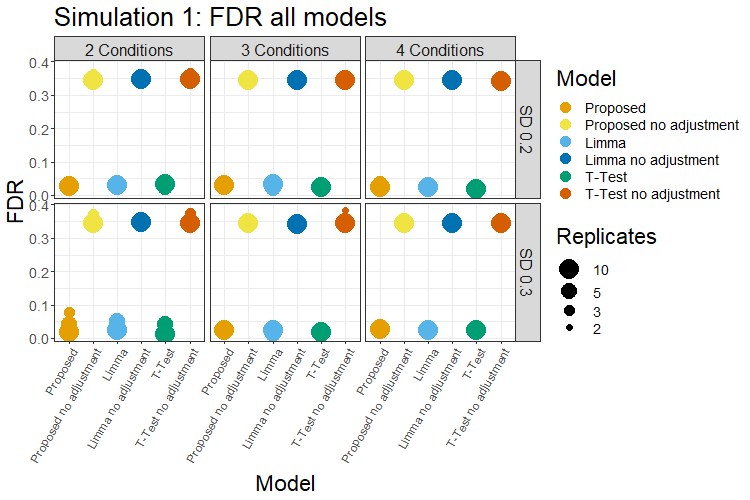
\includegraphics[width=.9\textwidth]{sim_new/sim1_FDR_all_models}\\
	\caption{All the considered methods in simulation 1 correctly calibrated FDR rate when adjusting for changes in protein abundance. In comparison, the methods without accounting for the protein-level changes resulted in off-target, high false positive rates.}
 \end{subfigure}
 \begin{subfigure}{.9\textwidth}
	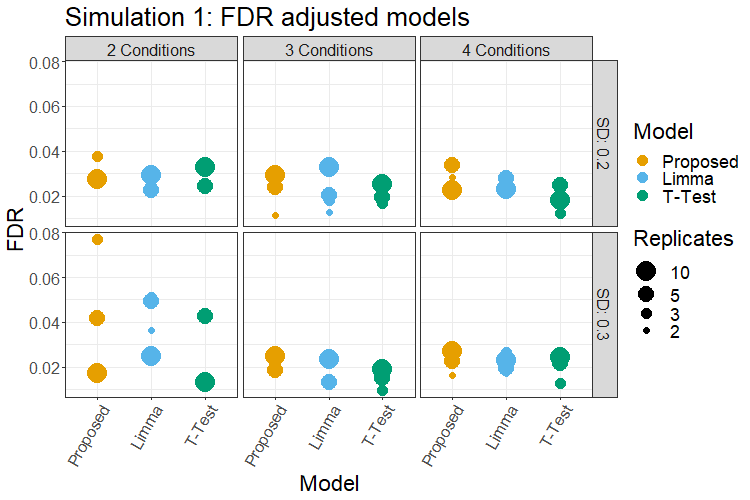
\includegraphics[width=.9\textwidth]{sim_new/sim1_FDR}
	\caption{The considered methods with protein adjustment are compared in detail. All three methods generally performed similarly in terms of FDR.}
 \end{subfigure}
\label{fig:sim1_fpr}
\end{figure}

\begin{figure}[h!]
\centering
 \begin{subfigure}{.9\textwidth}
	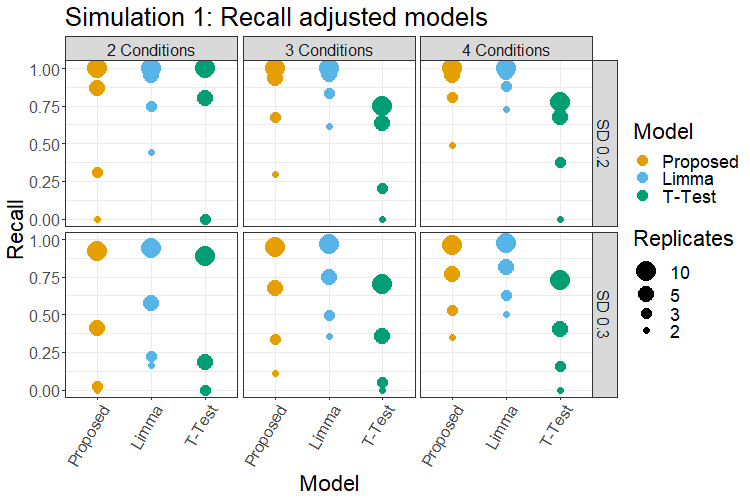
\includegraphics[width=.9\textwidth]{sim_new/sim1_Recall}\\
	\caption{The recall(false positive rate) for simulation 1 methods with adjustment were compared. It is clear that Limma performs the strongest here when the number of replicates were low.  At higher replicates the performance of the proposed methods and Limma are comparable. T-test clearly performs worse across all methods.}
 \end{subfigure}
 \begin{subfigure}{.9\textwidth}
	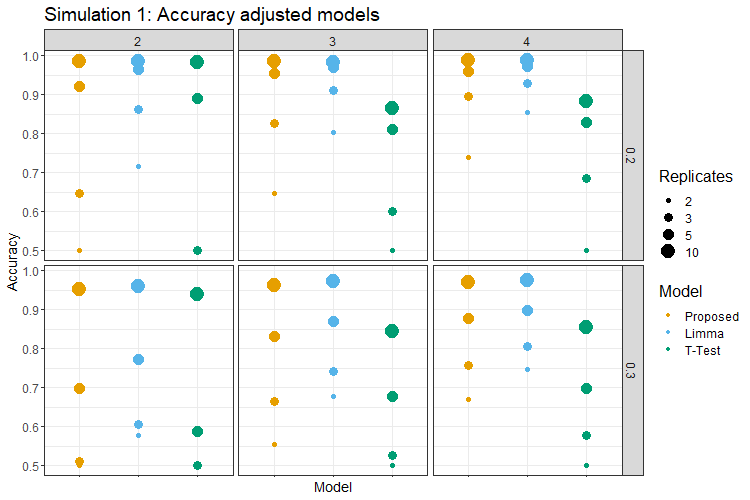
\includegraphics[width=.9\textwidth]{sim_new/sim1_accuracy}
	\caption{The overall accuracy plot mimics the observations in the recall plot. Limma performs stronger than the proposed method at lower replicates, while at higher they are comparable.}
 \end{subfigure}
\label{fig:sim1_recall}
\end{figure}

\begin{figure}[h!]
\centering
 \begin{subfigure}{.9\textwidth}
	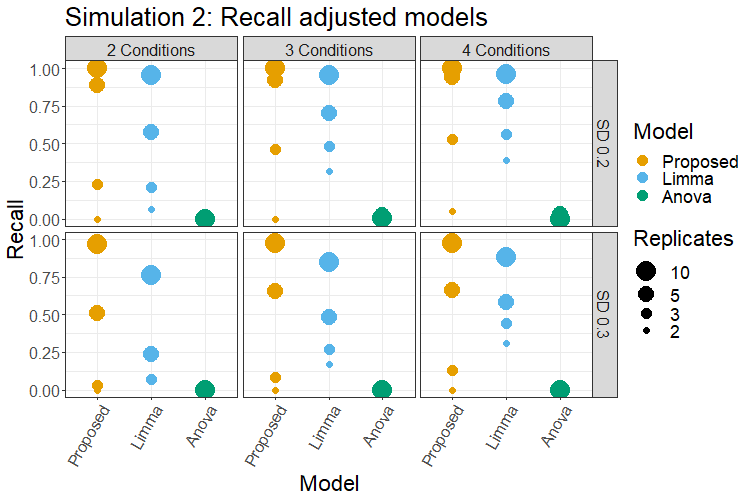
\includegraphics[width=.9\textwidth]{sim_new/sim3_Recall}
	\caption{The advantage of using the proposed approach is apparent when looking at simulation 2, which includes limited observations and the presence of missing values. In the case of recall the proposed method performs stronger than limma and t-test in nearly every model. Even at lower replicates the proposed method still outperformed limma, especially when there were more conditions in the simulation. Again the lowest performance was observed using the $t$-test method.}
 \end{subfigure}
 \begin{subfigure}{.9\textwidth}
	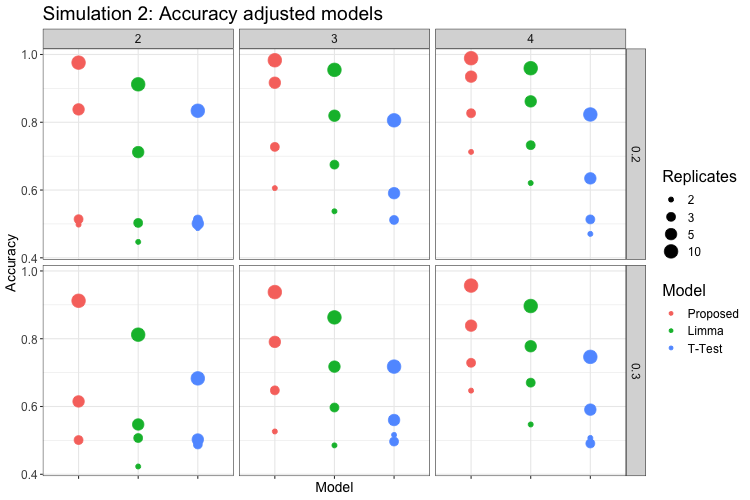
\includegraphics[width=.9\textwidth]{sim_new/sim3_Accuracy}
	\caption{The overall accuracy plots show similar results to recall. The proposed method performed the strongest across all methods, even when replicates were low. Limma shows strong performance in a clean experiment, when real world data problems are introduced it is clear the proposed method is more robust.}
 \end{subfigure}
\label{fig:sim2_recall}
\end{figure}

\begin{figure}[h!]
\centering
 \begin{subfigure}{.9\textwidth}
	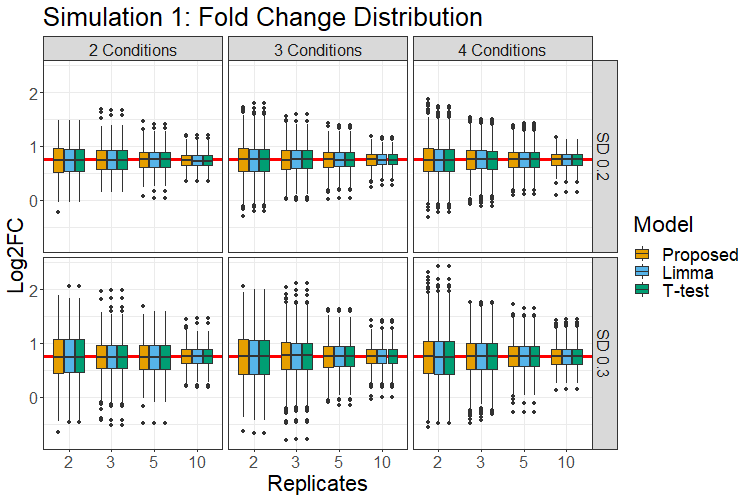
\includegraphics[width=.9\textwidth]{sim_new/sim1_FC_boxplot}
	\caption{In simulation 1 all considered methods correctly estimated the fold change between conditions, with a median fold change estimation of .75 in all methods. The distributions around the median were also consistent acorss all methods. Predictably the distribution quantiles decrease as the number of replicates increases.}
 \end{subfigure}
 \begin{subfigure}{.9\textwidth}
	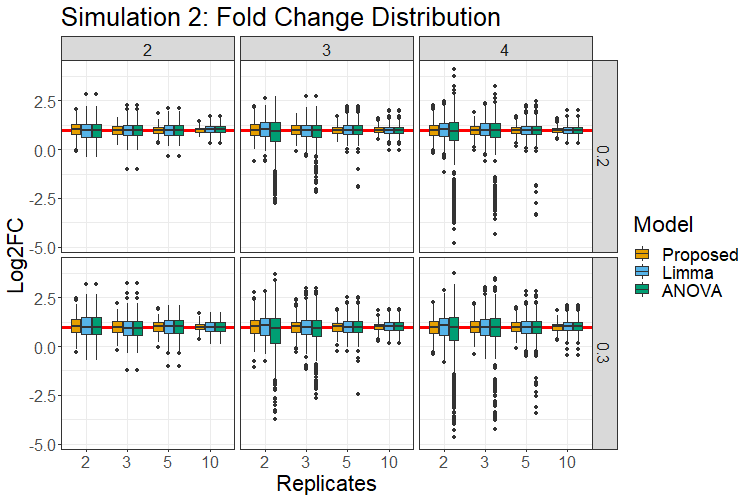
\includegraphics[width=.9\textwidth]{sim_new/sim3_FC_boxplot}
	\caption{In simulation 2 again all methods correctly estimated the fold change with a median log change of .75. The proposed method in this simulation had a visibly tighter distribution around the median. Both Limma and $t$-test showed a wider range around the fold change. In this case the proposed method showed a stronger performed in correctly estimating the fold change for all peptides.}
 \end{subfigure}
\label{fig:fc_boxplot}
\end{figure}

\clearpage
%%%%%%%%%%%%%%%%%%%%%%%%%%%%%%%%%%%%%%%%%%%%%%%%%%%%%%%%%%%%%%%%
\subsection{Benchmark experiment}
\label{sec:benchmark}

A custom designed experiment with labeling was used to assess the performance of the proposed method in a real experimental setting. Heavy-labeld KGG modified peptides were used as spike-in peptides. The spike-in peptides were mixed with human lysate to create four mixture conditions. Two sets of data were acquired for each mixture: KGG enriched + LC-MS, and LC-MS only. The KGG enriched dataset included the spike-in peptides, as well as modified and unmodified human lysate. The LC-MS dataset included only unmodified peptides. The spike-in peptides where a significant fold change between conditions are expected to be differencial, whereas none of the human lysate peptides in any comparison are expected to be differencial. 

Again we consider three different methods and assess their performance: the method proposed in this paper, Limma, and two sample $t$-test. All methods are analyzed after adjusting for changes in overall protein level. The propsed method summarizes feature intensities up to the run level using Tukey's Median Polish, while the other methods use the log of summed feature intensities. The results are summarized from \sfigref{fig:spike_volcano_msstats} to \sfigref{fig:spike_fc}, including volcano plots, model summary statsitics, and fold change analysis.

\begin{figure}[h!]
\centering
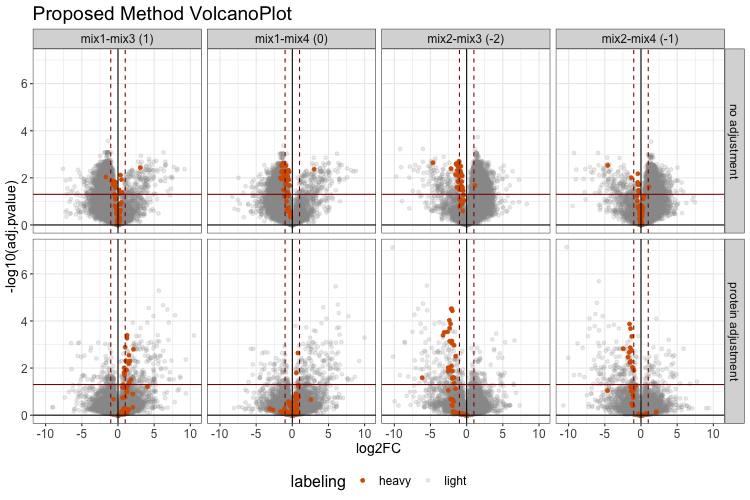
\includegraphics[width=.85\textwidth]{sim_new/spike_in_msstatsptm_volcano}
\caption{Using the proposed method to model the benchmark experiment the spike in peptides (colored red) do not follow the expected log fold change before adjustment. After adjusting for changes in overall protein abundance the spike in peptides are more in line with expectation. Additionally the background grey colored peptides showed many false positives before adjustment. After adjustment the false positives were decreased considerably. \label{fig:spike_volcano_msstats}}
\end{figure}

\begin{figure}[h!]
\centering
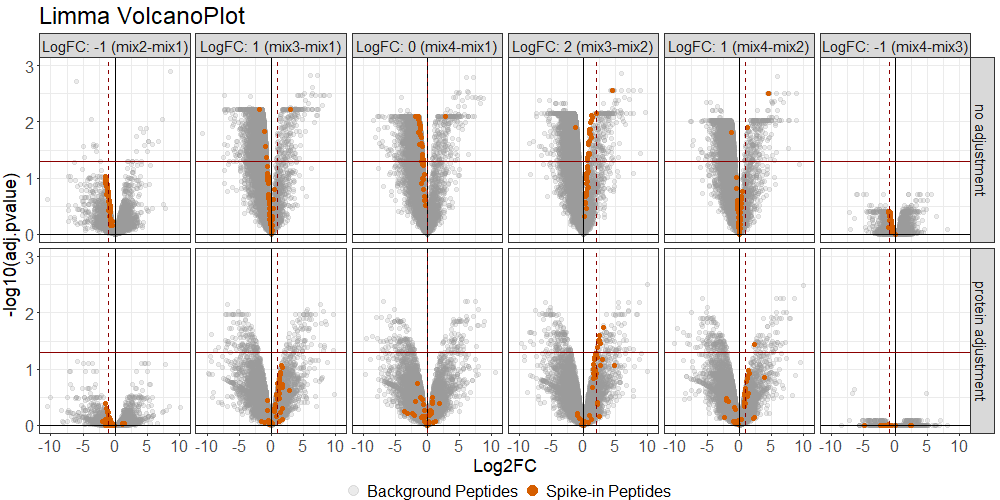
\includegraphics[width=.85\textwidth]{sim_new/spike_in_limma_volcano}
\caption{Using the limma method the spike in peptides follow the expected log fold change better after adjusting for changes in protein level. However, while the fold change is much more accurate, the majority of spike in peptides do not have a significante adjusted pvalue. In terms of false positives, the results are very similar to the propsed method, with many false positives before adjustment and much fewer afterward. \label{fig:spike_volcano_limma}}
\end{figure}

\begin{figure}[h!]
\centering
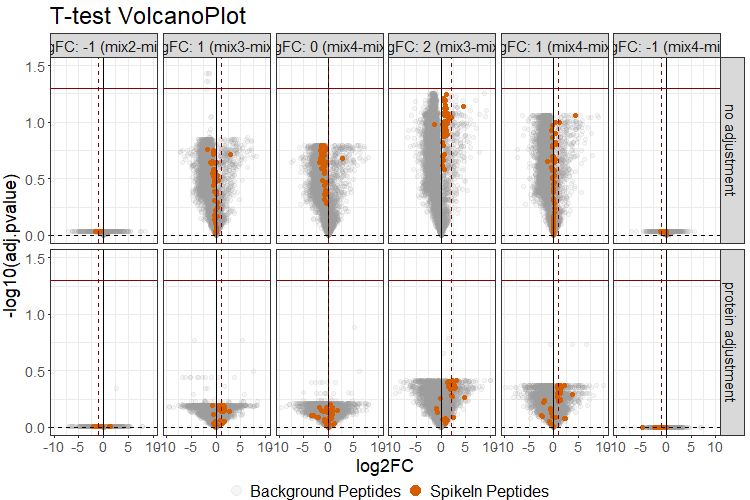
\includegraphics[width=.85\textwidth]{sim_new/spike_in_ttest_volcano}
\caption{Using the two sample $t$-test, none of the comparisons either before or after adjustment do not show any significant peptides. With that being said, the fold change of the spike in peptides is much closer to expectation after adjusting for global protein abundance. \label{fig:spike_volcano_ttest}}
\end{figure}

\begin{figure}[h!]
\centering
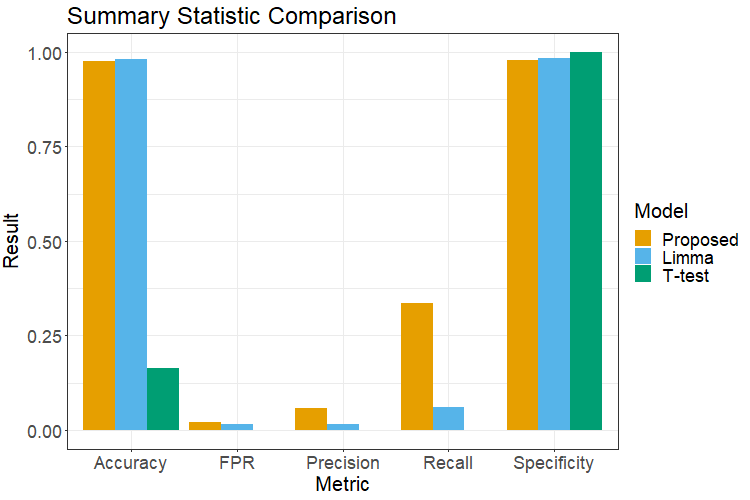
\includegraphics[width=.85\textwidth]{sim_new/spike_in_statistic_comparison}
\caption{Comparing the summary statistics between methods it is clear that the proposed method performs the strongest. In terms of accuracy and specificity the three methods are close, with Limma and $t$-test showing slightly higher values. Accuracy and specificity are dominated by the large number of true negatives (background peptides) compared to the true positives (spike in peptides). In terms of recall, the proposed approach far out performed the other two methods, showing that it correctly labeled the most spike in peptides. \label{fig:spike_stat}}
\end{figure}

\begin{figure}[h!]
\centering
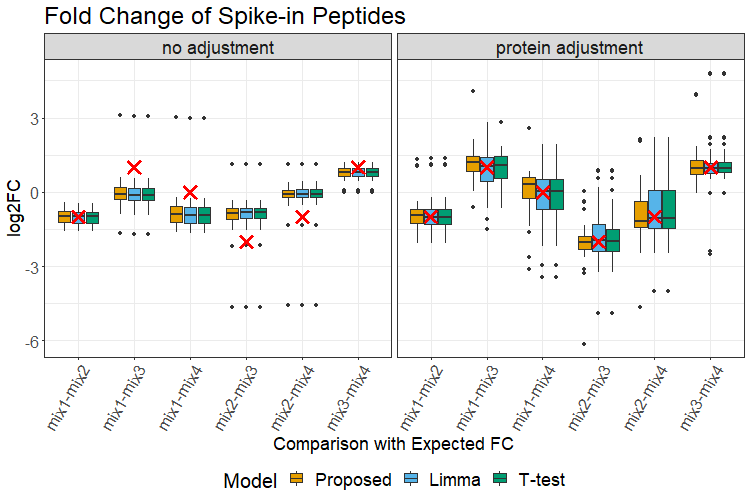
\includegraphics[width=.85\textwidth]{sim_new/spike_in_fc}
\caption{The fold change misalignment before adjustment is illustrated in the boxplots. The true log fold change is indicated by the red 'X' marks. Before adjustment the boxplots are not close to the true fold change. After adjustment all three models generally have median near the true fold change. In terms of model comparison, the proposed method shows a much tighter distribution around the true fold change, whole both Limma and $t$-test are much wider. \label{fig:spike_fc}}
\end{figure}


\clearpage
%%%%%%%%%%%%%%%%%%%%%%%%%%%%%%%%%%%%%%%%%%%%%%%%%%%%%%%%%%%%%%%%
\section{Datasets : Biological investigation}

\subsection{IpaH7.8}

In this experiment Shigella ubiquitin ligase IpaH7.8 was shown to inhibit the protein gasdermin D (GSDMD). Multiplex proteomics was used to quantify the abundance of total protein, and ubiquitination in human epithelial cells. Cells were either infected or uninfected with IpaH7.8-deficient Shigella flexneri and measurements were taken at different time periods. Uninfected cells were measured at 0 and 6 hours, while infected cells were measured at 1, 2, 4, and 6 hour increments, resulting in six total conditions. The experiment was inbalanced with two bioreplicates per condition for all conditions except for infected 1 hour. The experimental design can be seen in Table~\ref{table:ipah_design}.

\begin{table}[h!]
\centering
\begin{tabular}{| c | c | c |}
\hline
 Condition & BioReplicate & Channel \\ [0.5ex]
 \hline\hline
 Dox1hr & Dox1hr\_1 & 127C\\
 \hline
 Dox2hr & Dox2hr\_1 & 128N\\
\hline
 Dox2hr & Dox2hr\_2 & 130C\\
\hline
 Dox4hr & Dox4hr\_1 & 128C\\
\hline
 Dox4hr & Dox4hr\_2 & 131C\\
\hline
 Dox6hr & Dox6hr\_1 & 129N\\
\hline
 Dox6hr & Dox6hr\_2 & 131N\\
\hline
 NoDox0hr & NoDox0hr\_1 & 126C\\
\hline
 NoDox0hr & NoDox0hr\_2 & 129C\\
\hline
 NoDox6hr & NoDox6hr\_1 & 127N\\
\hline
 NoDox6hr & NoDox6hr\_2 & 130N\\
\hline

\end{tabular}
\caption{The experimental design of the IpaH7.8 experiment}
\label{table:ipah_design}
\end{table}

A model was fit for the total protein, and ubiquitination separately, as described previously for TMT experiments in Section~\ref{sec:tmtmethod}. The model formula can be seen below.

\todo{only one mixture so we probably wouldn't include the mixture as a term in the model?}

$$Y_{mcb} = \mu + Condition_c + Subject_{mcb} + \epsilon_{mcb}$$

$$\sum_{c=1}^C{Condition_c} = 0 ,\: Subject_{mcb} ~ \sim N(0, \sigma^2_S) ,\: \epsilon_{mcb} ~ \sim N(0, \sigma^2)$$

The results of the proposed method to this experiment can be seen in \sfigref{fig:ipah_figures}.

\begin{figure}[h!]
\centering
 \begin{subfigure}{\textwidth}
	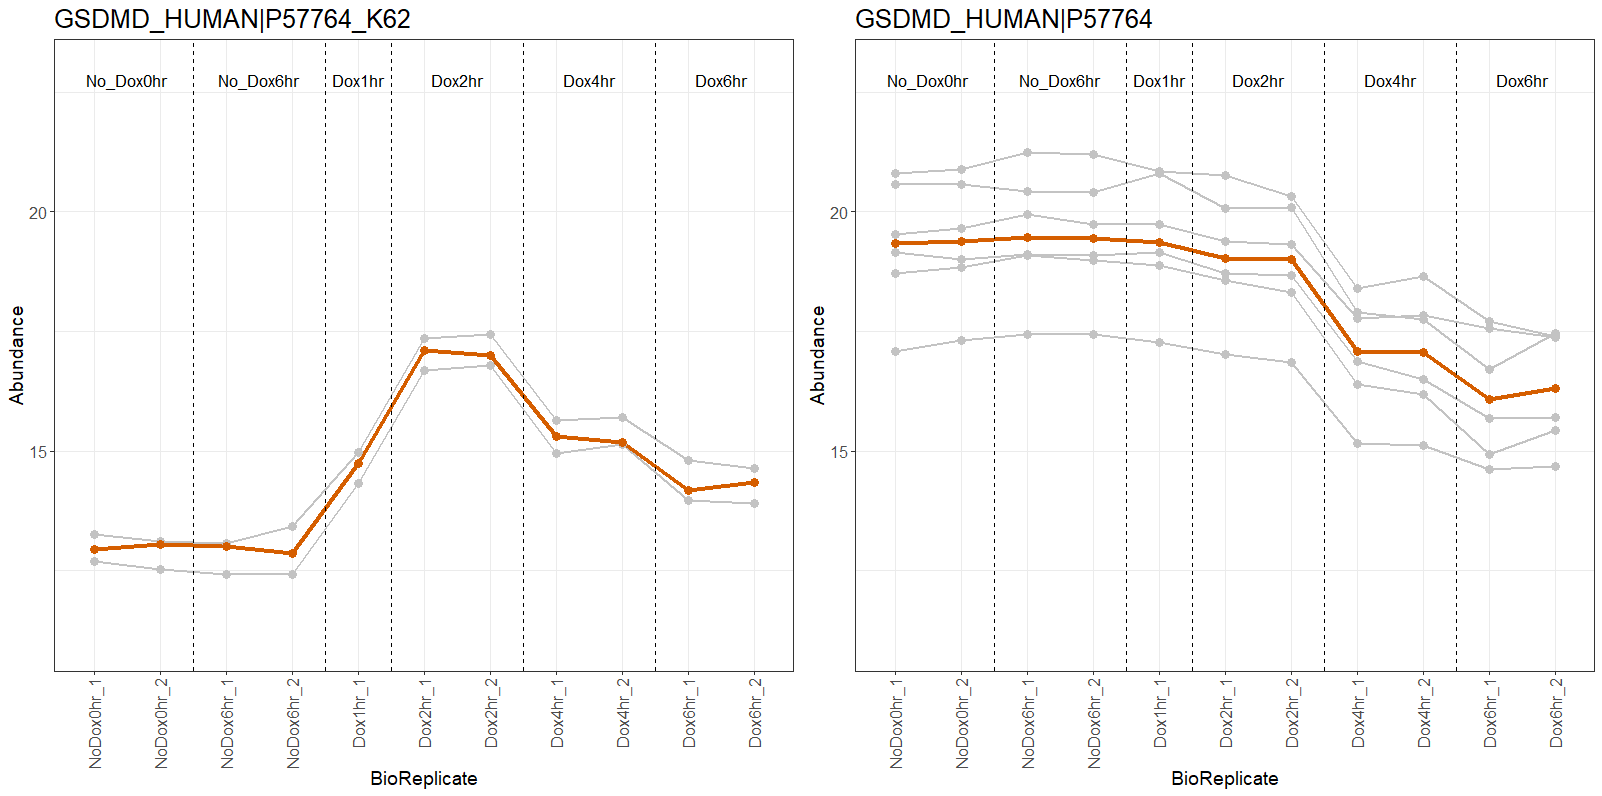
\includegraphics[width=\textwidth]{sim_new/IpaH_prof_plot}
	\caption{Comparing the global profiling of protein $GSDMD\_HUMAN|P57764$ with the ubiquitination of the protein at site $K62$. The individual PSM features are shown in grey, while the feature summarization is shown in red. When looking at the summary of the modification and global protein it is clear the conditions follow different trends. Specifically, there appears to be no change in abundance between Dox1hr and Dox4hr in the modified plot, however there is a large negative change when looking at the unmodified plot. This indicates the modification is confounded with changes in the unmodified protein.}
 \end{subfigure}
 \begin{subfigure}{\textwidth}
	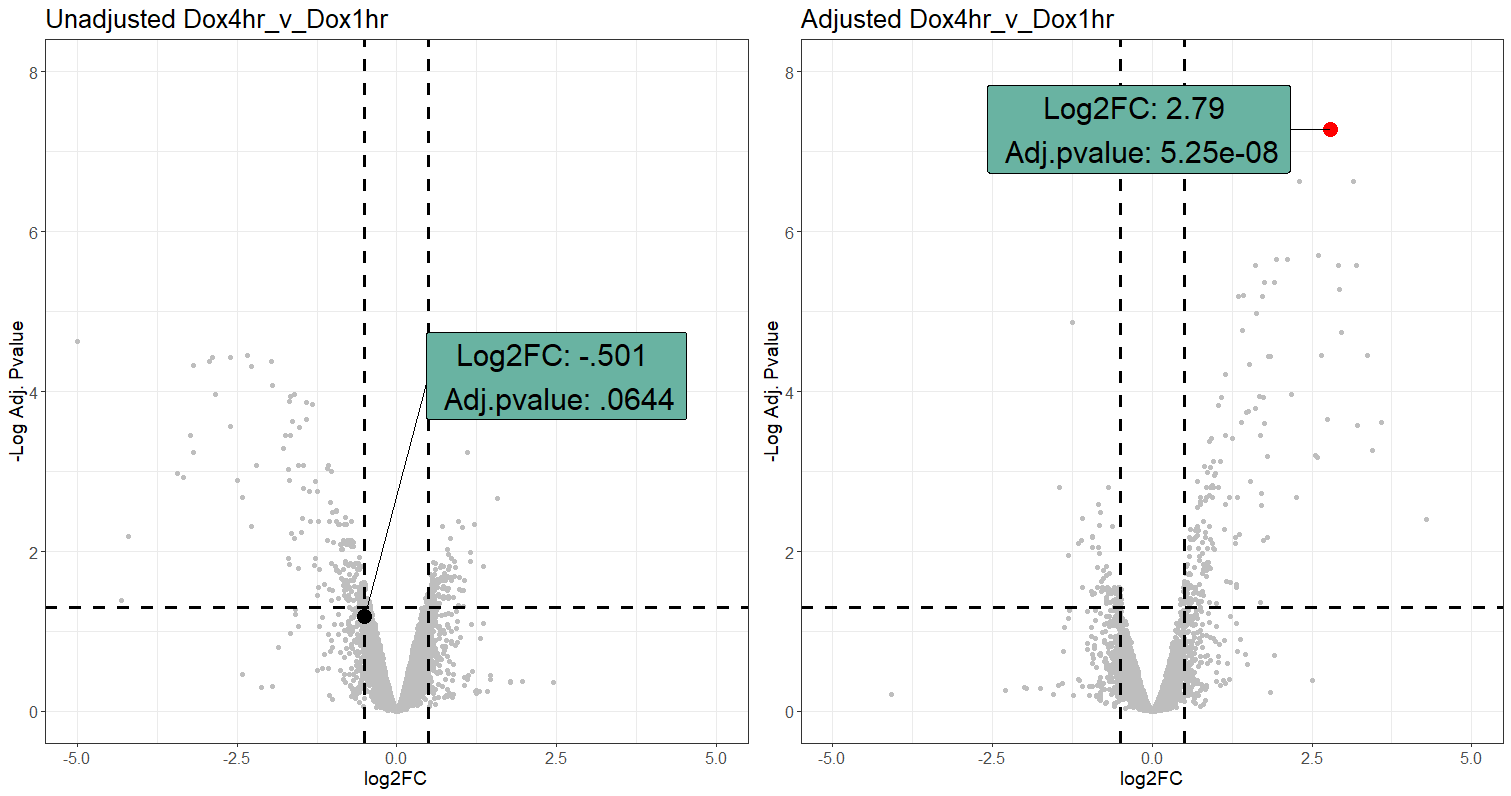
\includegraphics[width=\textwidth]{sim_new/IpaH_volcano_plot}
	\caption{Volcano plots of Dox4hr vs Dox1hr both before and after protein adjustment. The $GSDMD\_HUMAN|P57764\_K62$ modification is highlighted. Before adjustment the modification has a small fold change and insignificant adjusted pvalue. After adjustment the fold change is much larger and the adjusted pvalue is very significant. In this case the proposed method allows us to identify differential modified peptides that could have otherwise been missed.}
 \end{subfigure}
\label{fig:ipah_figures}
\end{figure}

\clearpage
\subsection{Shigella flexneri}

In this study, the correlation between the gene Atg16L1 and killing of Shigella flexneri (S.flexneri) was assessed. Multiplex proteomics was used to quantify the abundance of total protein, phosphorylation, and ubiquitination in wild type (WT) and ATG16L1-deficient (cKO) samples, uninfected and uninfected with S.flexneri. The abundance of total protein and post-translation modifications were quantified at three time points, uninfected, early infection (45-60 minutes), and late infection (3-3.5 hours). Quantifying the total protein along with the post-translational modifications allowed us to adjust for changes in total protein and see the true impact of the site specific modifications. Two mixtures using 11-plex were ran over the six conditions. The six conditions were split between 11 channels leading to the experimental design being unbalanced. Each mixture contained two replicates per early and late WT and KO conditions. Mixture one contained one replicate of uninfected WT and two replicates of uninfected KO. Mixture two contained one replicate of uninfected KO and two uninfected WT. The experimental design can be seen in Table~\ref{table:shigella_design}.

\begin{table}[h!]
\centering
\begin{tabular}{|c | c c | c c | c|}
\hline
 & Mixture 1 & & Mixture 2 & & Condition \\ [0.5ex]
 \hline\hline
 Uninfected & 128C & & 128C & 131C & \\
 \hline
Early (1 Hour) & 126C & 129C & 126C & 129C & WT \\
\hline
Late (3 Hour) & 127C & 130C & 127C & 130C & \\
\hline
Uninfected & 129N & 131C & 129N & & \\
\hline
Early (1 Hour) & 127N & 130N & 127N & 130N & KO \\
\hline
Late (3 Hour) & 128N & 131N & 128N & 131N & \\
\hline

\end{tabular}
\caption{The experimental design of the Shigella flexneri experiment}
\label{table:shigella_design}
\end{table}

A model was fit for the total protein, phosphorylation, and ubiquitination separately, as described previously for TMT experiments. The model formula can be seen below.

$$Y_{mcb} = \mu + Mixture_m + Condition_c + Subject_{mcb} + \epsilon_{mcb}$$

$$Mixture_m ~ \sim N(0, \sigma^2_M) ,\: \sum_{c=1}^C{Condition_c} = 0 ,\: Subject_{mcb} ~ \sim N(0, \sigma^2_S) ,\: \epsilon_{mcb} ~ \sim N(0, \sigma^2)$$

The results of the proposed method to this experiment can be seen in \sfigref{fig:No_Diff_Shigella_PTM} and \sfigref{fig:Diff_Shigella_PTM}.


\begin{figure}[h!]
\centering
 \begin{subfigure}{\textwidth}
	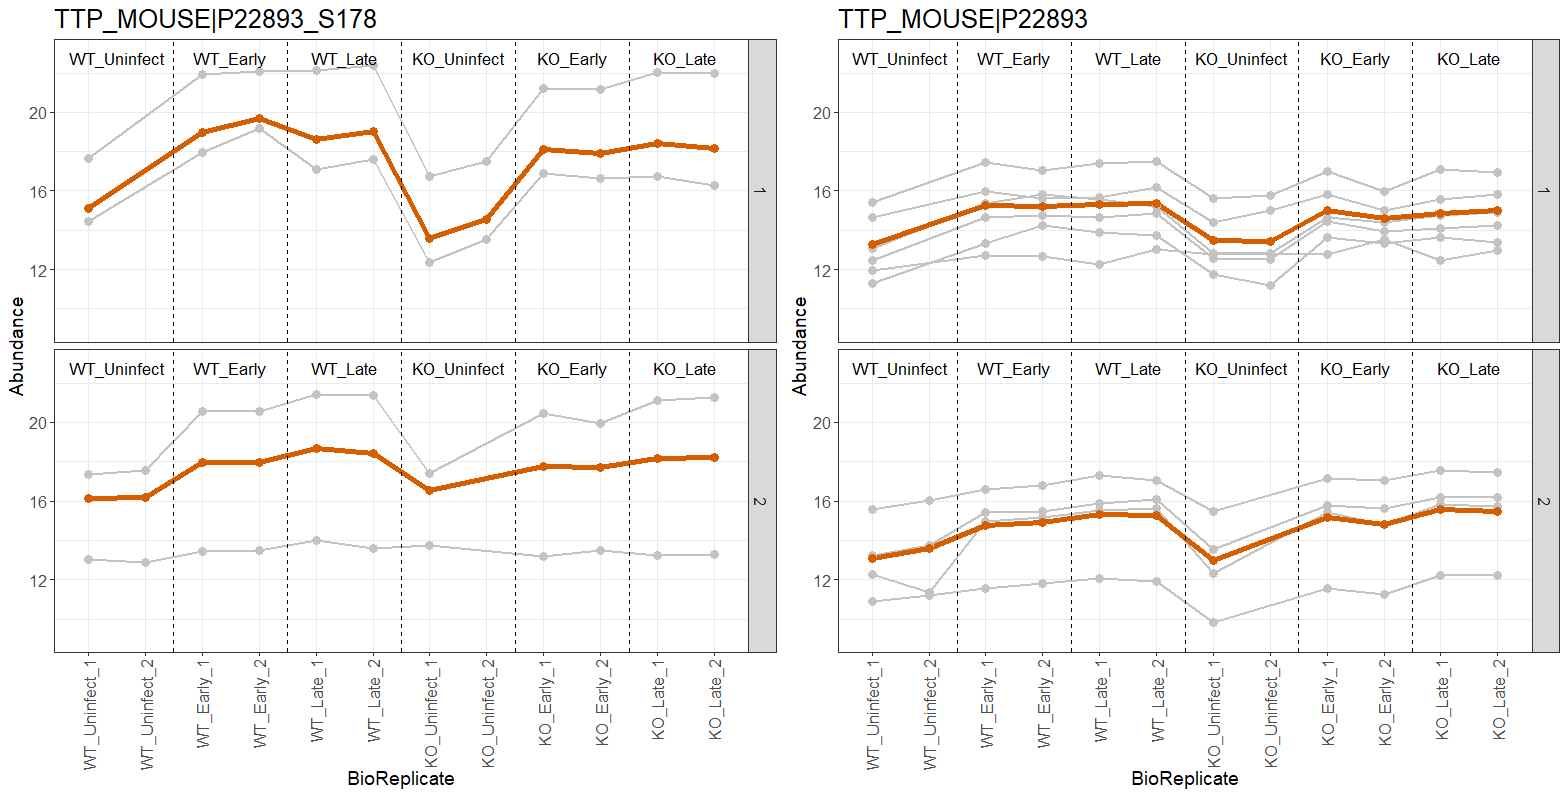
\includegraphics[width=\textwidth]{sim_new/No_Difference_Shigella_Profile_Plot}
	\caption{Comparing the global profiling of protein $TTP\_MOUSE|P22893$ with the modification of the protein at site $S178$. The individual PSM features are shown in grey, while the feature summarization is shown in red. When looking at the summary of the modification and global protein it is clear the difference between conditions follow the same trend. Specifically, there is a positive adjustment in abundance when comparing WT\_Uninfect to WT\_Late in both the modification and global profiling run. This indicates the movement is driven by changes in global protein.}
 \end{subfigure}
 \begin{subfigure}{\textwidth}
	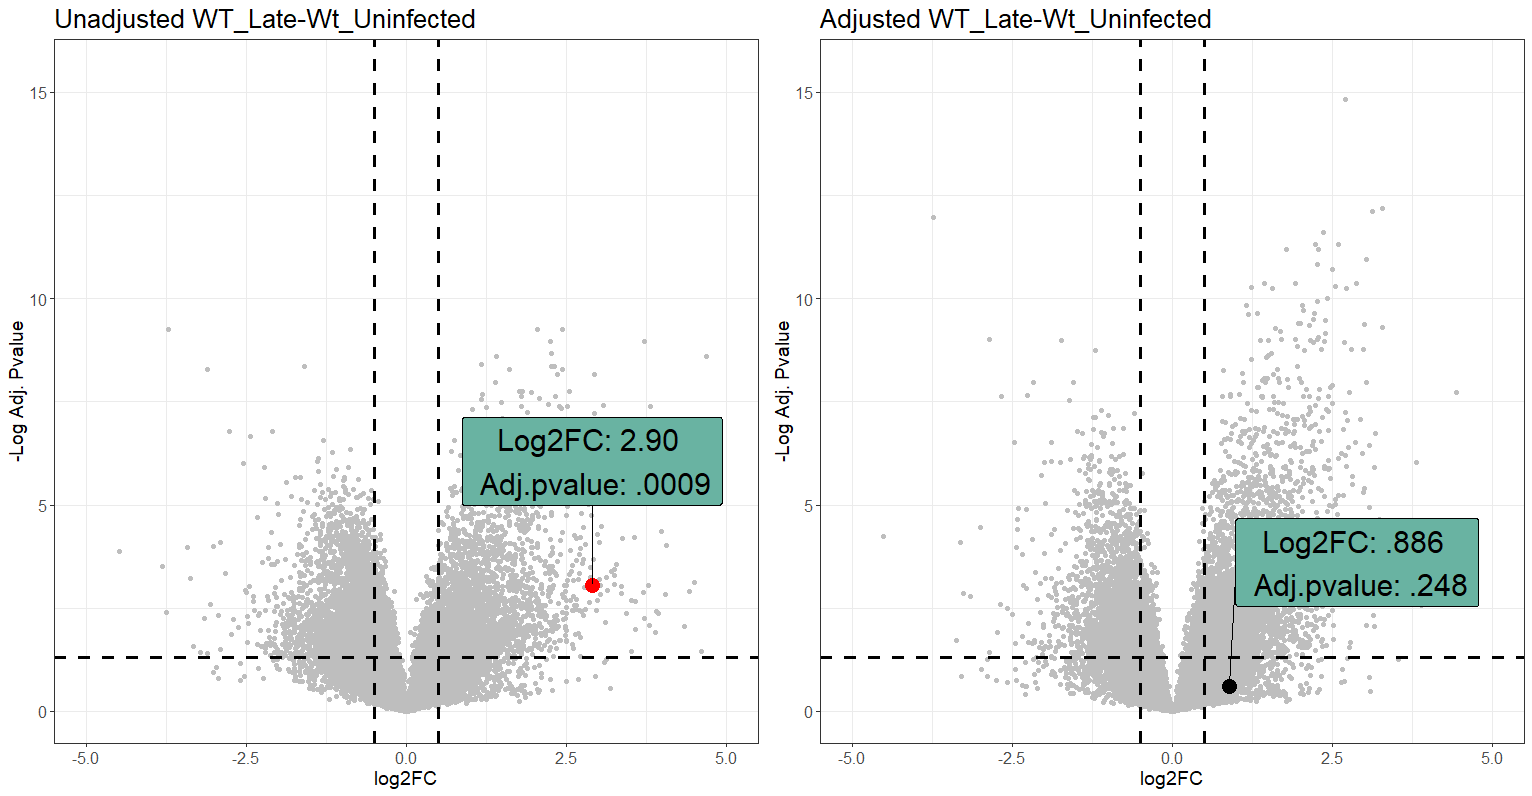
\includegraphics[width=\textwidth]{sim_new/No_Difference_Shigella_Volcano}
	\caption{Volcano plots of WT\_Late vs WT\_Uninfect both before and after protein adjustment. The $TTP\_MOUSE|P22893\_S178$ modification is highlighted. Before adjustment the modification has a large fold change and significant adjusted pvalue. After adjustment the fold change is much smaller and the adjusted pvalue is insignificant.}
 \end{subfigure}
\label{fig:No_Diff_Shigella_PTM}
\end{figure}

\begin{figure}[h!]
\centering
 \begin{subfigure}{\textwidth}
	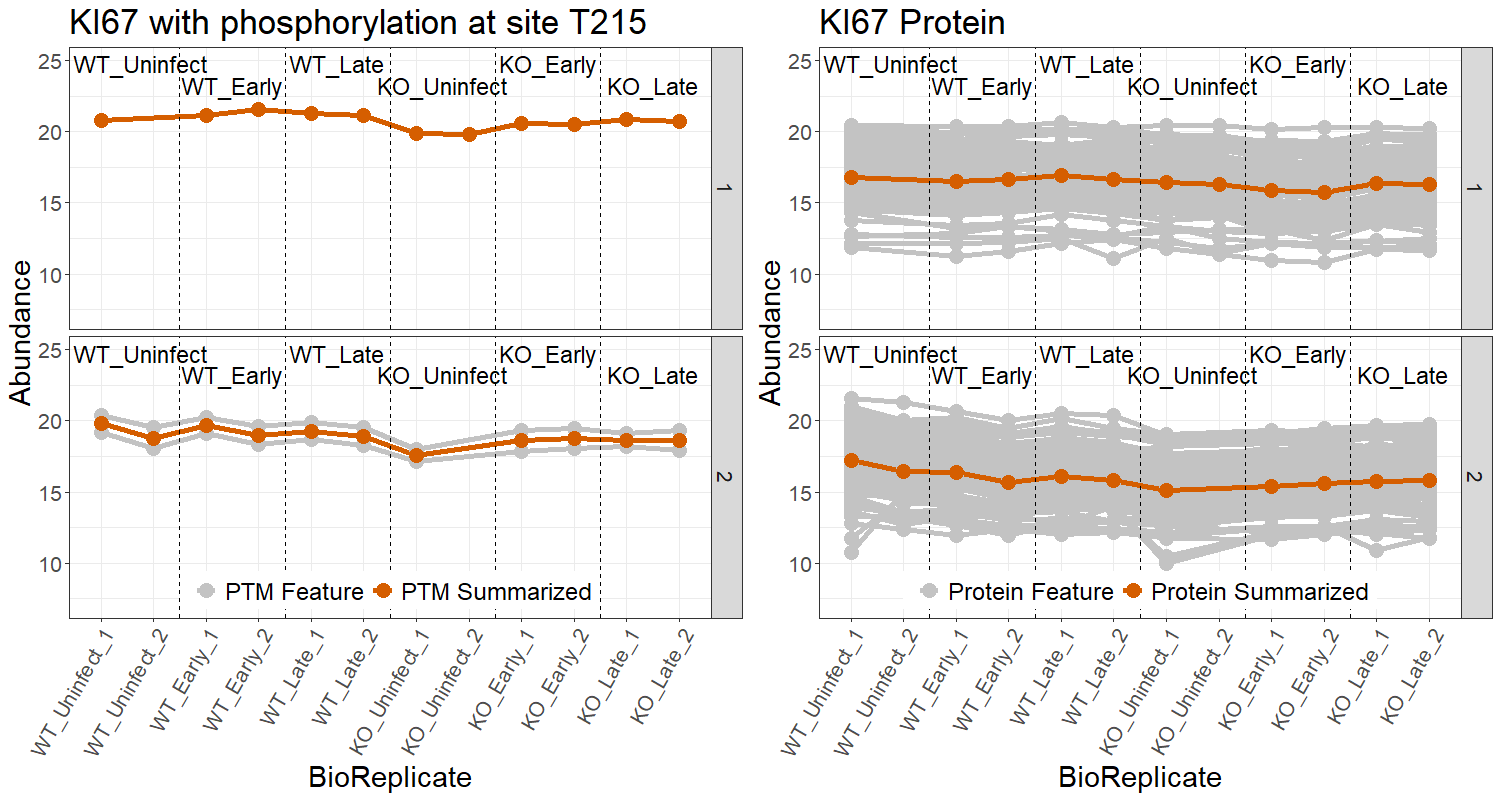
\includegraphics[width=\textwidth]{sim_new/Difference_Shigella_Profile_Plot}
	\caption{Comparing the global profiling of protein $KI67\_MOUSE|E9PVX6$ with the modification of the protein at site $T215$. In this case the modification and global protein trend in different directions. Specifically, comparing WT\_Uninfect and WT\_Early there is a slightly positive change in abundance, however in the global profiling there was a negative change. In this case the profile plot indicates the effect of the modification is masked by the change in global protein abundance. Additionally this profile plot shows the large difference in available features between modifications and global protein.}
 \end{subfigure}
 \begin{subfigure}{\textwidth}
	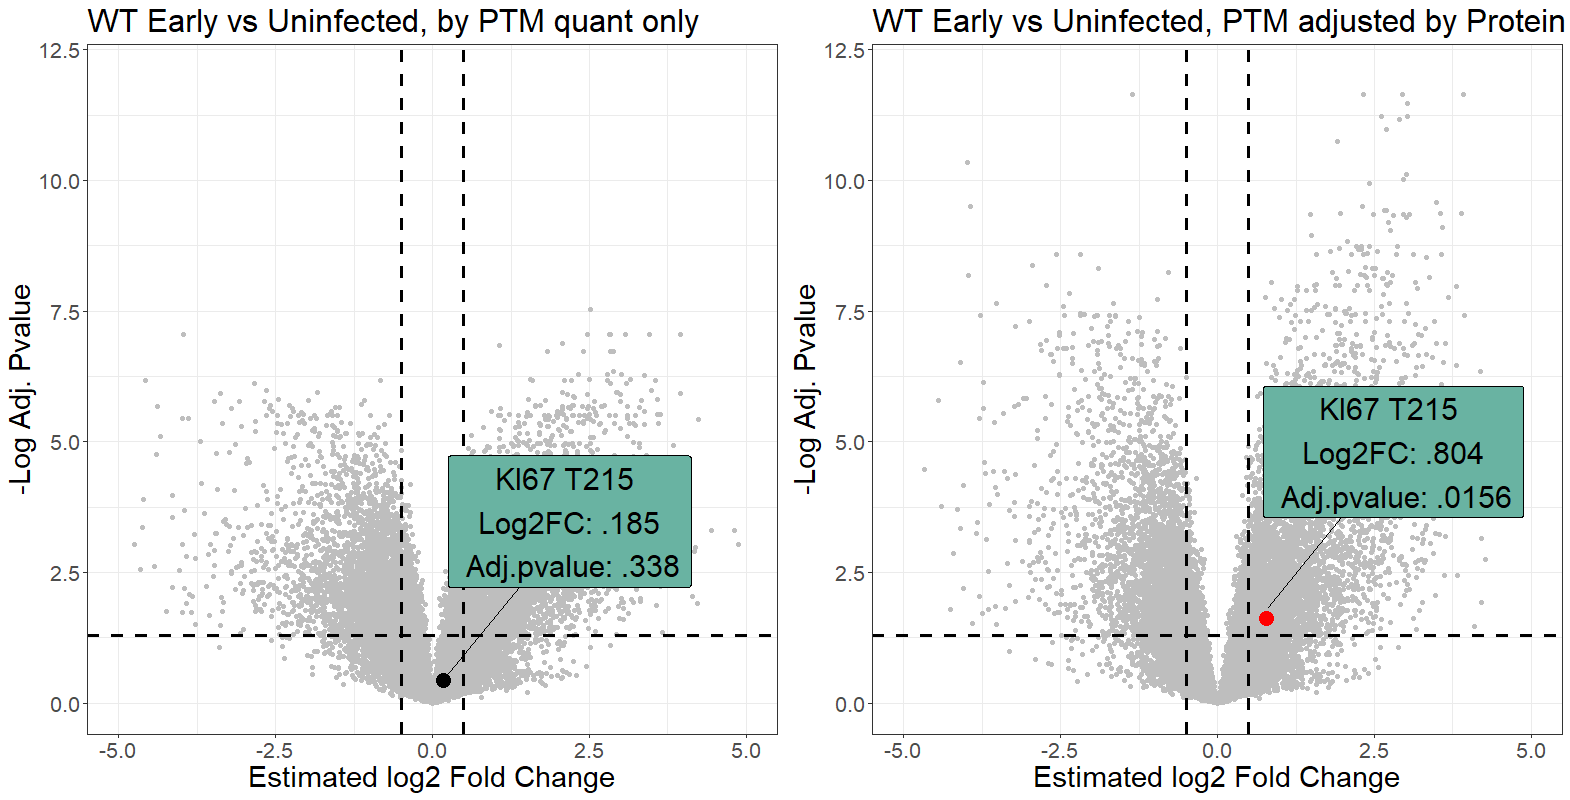
\includegraphics[width=\textwidth]{sim_new/Difference_Shigella_Volcano}
	\caption{Volcano plots of WT\_Early vs WT\_Uninfect both before and after protein adjustment. The $KI67\_MOUSE|E9PVX6$ modification is highlighted. Before adjustment the modification has a small positive fold change and insignificant adjusted pvalue. After adjustment the fold change increases and the adjusted pvalue is now significant.}
 \end{subfigure}
\label{fig:Diff_Shigella_PTM}
\end{figure}

\clearpage

\subsection{USP30}

This experiment looked into the relationship between USP30 and protein kinase PINK1, and their association with Parkinson's Disease. Ubiquitination site profiling was performed and the modified site abundance was analyzed. Four conditions were tested with two biological replicates per condition. The conditions were as follows: CCCP, USP30 overexpression (USP30\_OE), Combo, and Control. Label-free mass spectrometry quantification was used to quantify the abundance of modified peptides. A corresponding mixed effects model was fit per modification and global protein as described previously in this supplementary.

In contrast to other experiments analyzed in this paper, there was no unmodified global protein profiling run performed in this experiment. Once identification and quantification of the Ubiquitinated profiling was performed, peptides which were unmodified were extracted and used in place of a global profiling run. This resulted in a significant lack of overlap between modified and unmodified peptides. Any modified peptide without a corresponding unmodified protein could not be adjusted. Of the 10,799 modified peptides identified, only 4526 had a corresponding unmodified run and could be adjusted. Finally, using this method also resulted in a low feature count for the unmodified protein model.

An example profile plot for this experiment can be seen in \sfigref{fig:USP30_profile_plot}.

\begin{figure}[h!]
\centering
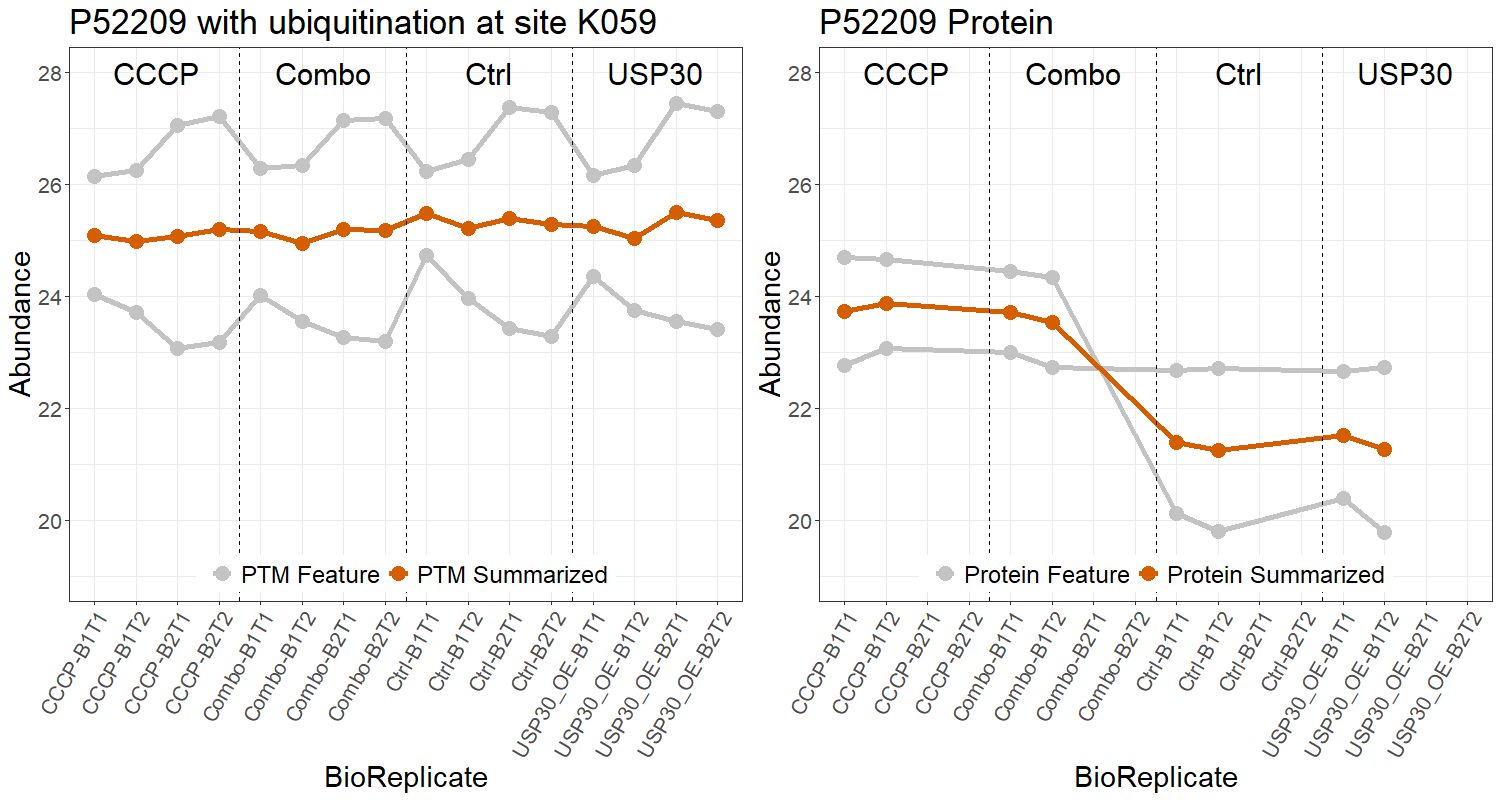
\includegraphics[width=\textwidth]{sim_new/USP30_profile_plot}
\caption{Comparing the global profiling of protein $P52209$ with the modification of the protein at site $K059$. The modification appears generally unchanged between conditions, whereas the global profiling run shows the CCCP and Combo conditions at a higher relative abundance compared to the Control and USP30\_OE. This indicates that the modification actually had a major effect when comparing CCCP and Combo to Control and USP30\_OE, which would have been missed without adjusting for global protein changes.}
\label{fig:USP30_profile_plot}
\end{figure}
\clearpage
%%%%%%%%%%%%%%%%%%%%%%%%%%%%%%%%%%%%%%%%%%%%%%%%%%%%%%%%%%%%%%%%
\section{Sample size calculation and power analysis}

The proposed approach allows us to calculate the sample size needed to achieve a desired statistical power as described in Section \ref{sec:design}. Given a desired power of .9, varying standard deviations, and an expected fold change, the number of replicates per condition can be seen in \sfigref{fig:sample_size}

\begin{figure}[h!]
\centering
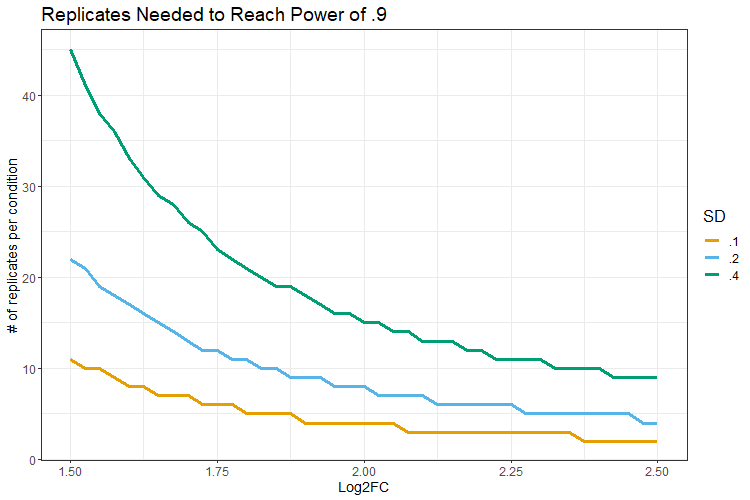
\includegraphics[width=\textwidth]{sim_new/simple_power_analysis}
\caption{The number of replicates per condition required to reach a power of .9 can be seen in the plot. At a high standard deviation and low expected fold change the number of replicates is unrealistically high. As the expected fold change increases the number of replicates needed decreases dramatically. The standard deviation of .1 expectantly shows the least number of replicates needed regardless of fold change.}
\label{fig:sample_size}
\end{figure}


As described in Section \ref{sec:test} the proposed method adjusts for the underlying protein abundance in the PTM significance analysis, which corrects the confounding factor with a cost of increased variation. When the variation is increased, the experiment requires a larger number of replicates to reach the same power. 

We compared the required sample size with varying standard deviations for the modified and unmodified peptide models. Three pairs of standard deviations of log-intensities for modified and unmodified peptides were used: (0.2, 0.1), (0.2, 0.2), and (0.2, 0.4). In the first pair the standard deviation for the unmodified peptide was less than the modified, in the second the standard deviations are the same, and in the third the standard deviation for the unmodified peptide was more than for the modified peptide. Again the desired power was .9 and the expected fold change was varied. The results can be seen in \sfigref{fig:power_sd_combo}

\begin{figure}[h!]
\centering
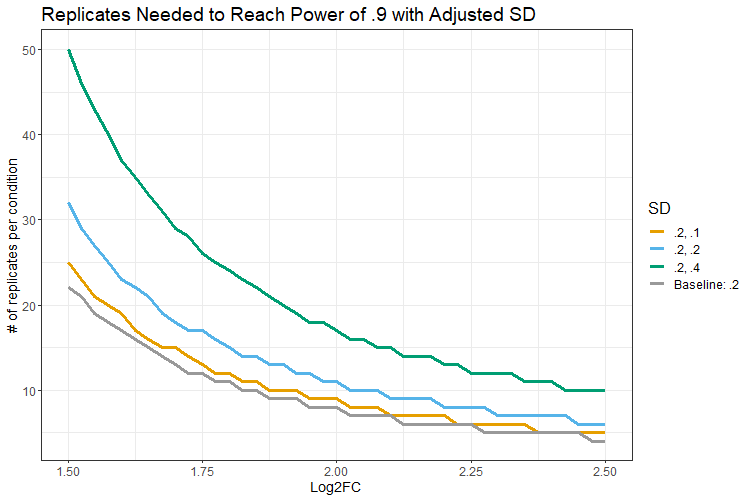
\includegraphics[width=\textwidth]{sim_new/power_analysis_sd_combined}
\caption{When the unmodified peptide has a low standard deviation the number of replicates is very similar to the baseline. As the standard deviation increases the number of replicates increases greatly. When the unmodified stand deviation is much higher than the modified, we can see that many more replicates are needed to reach the same power.}
\label{fig:power_sd_combo}
\end{figure}

%\begin{figure}[h!]
%\centering
%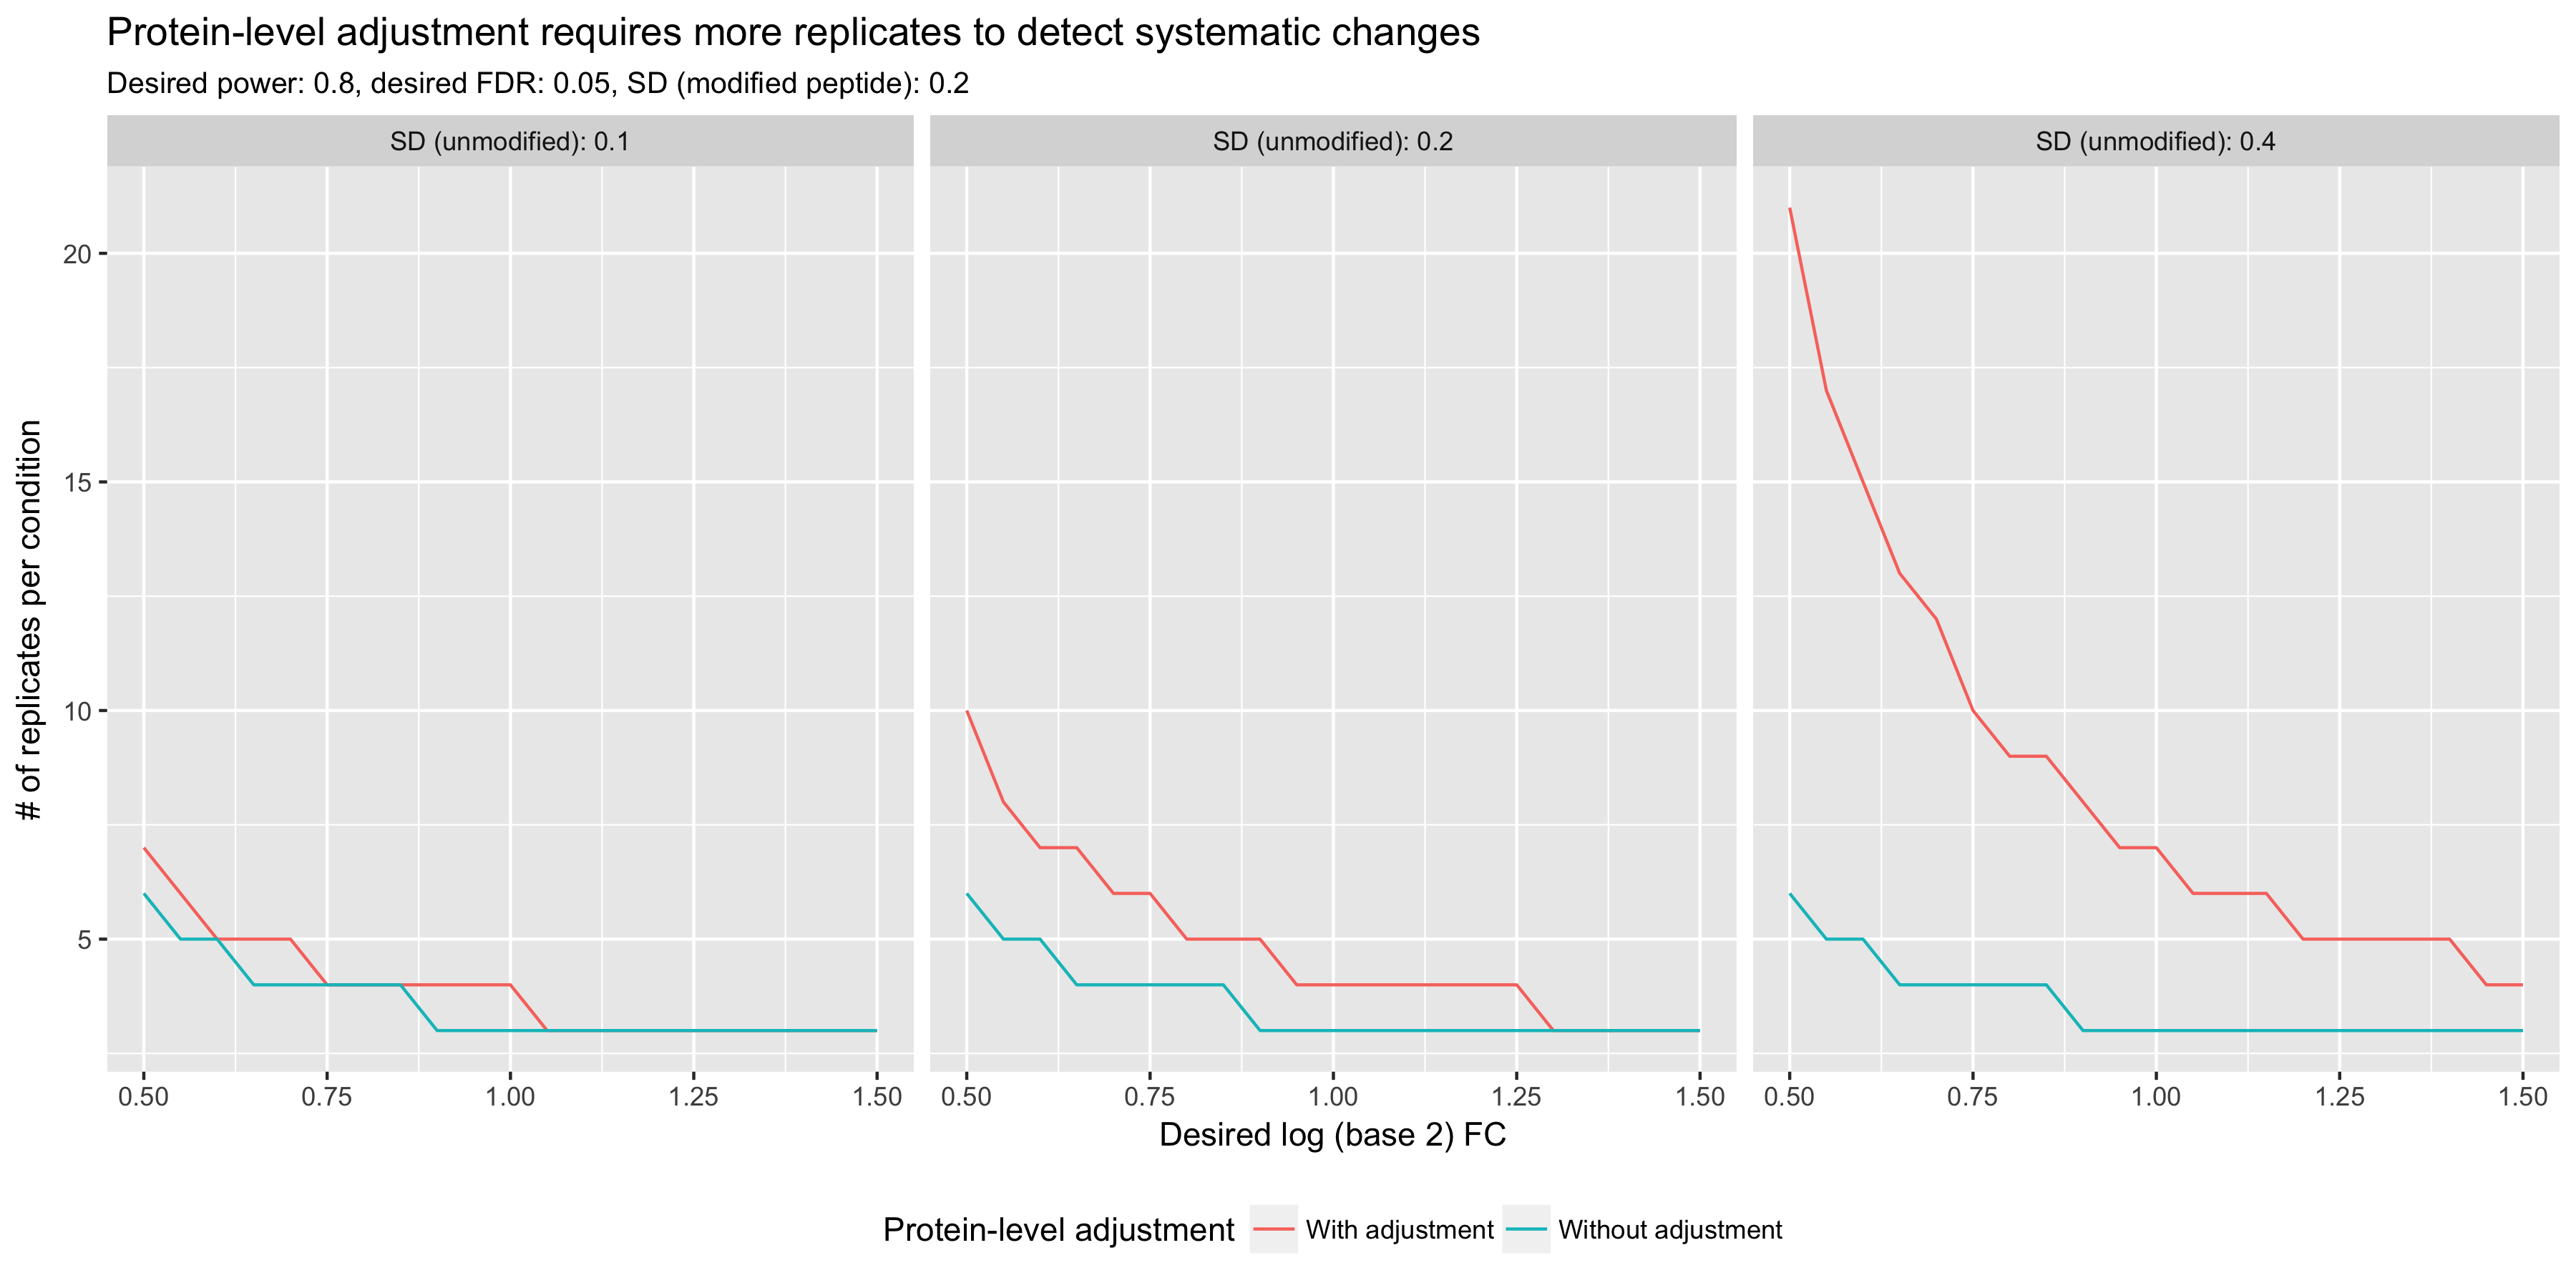
\includegraphics[width=\textwidth]{sim/size_prot}
%\caption{Protein-level adjustment relies on the inference of protein abundance, %which introduces additional uncertainty in the estimate of PTM difference. %Therefore, the required sample size to detect a systematic change is higher than as %expected for standard differential analysis without adjustment. The discrepancy can %be profound if the uncertainty associated with the protein abundance estimate is %greater than that of PTM abundance estimate. Sample size calculation without %accounting for the uncertainty would lead to under-powered studies. %\label{fig:size_prot}}
%\end{figure}

%\begin{figure}[h!]
%\centering
%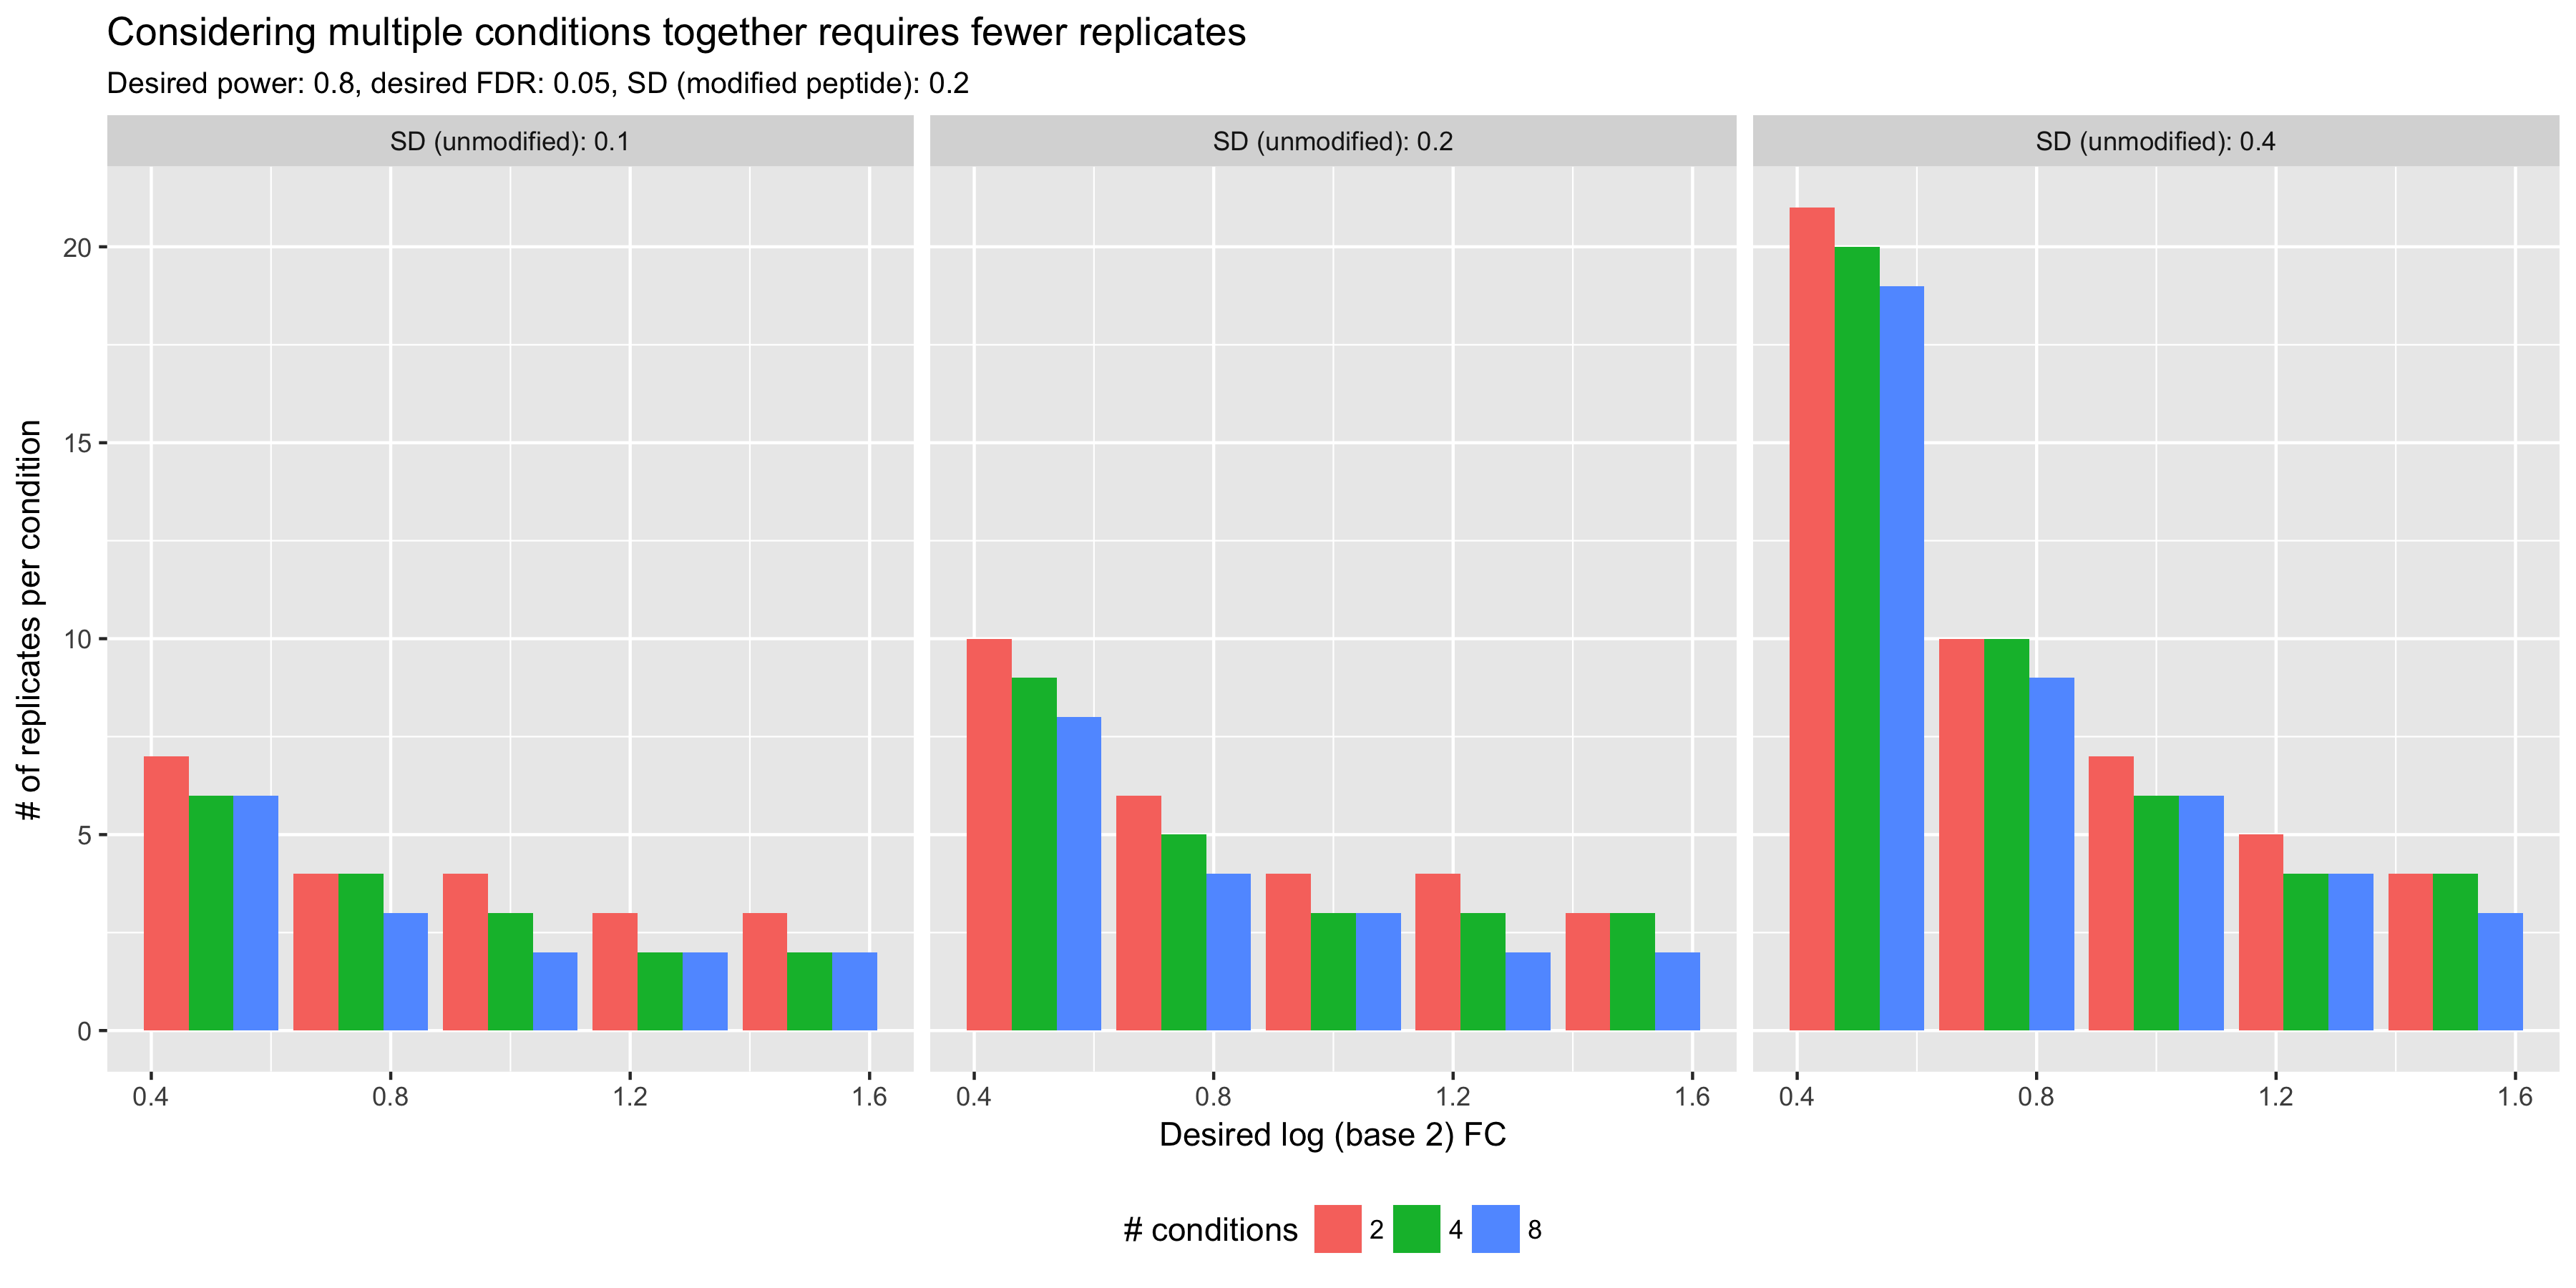
\includegraphics[width=\textwidth]{sim/size_grp}
%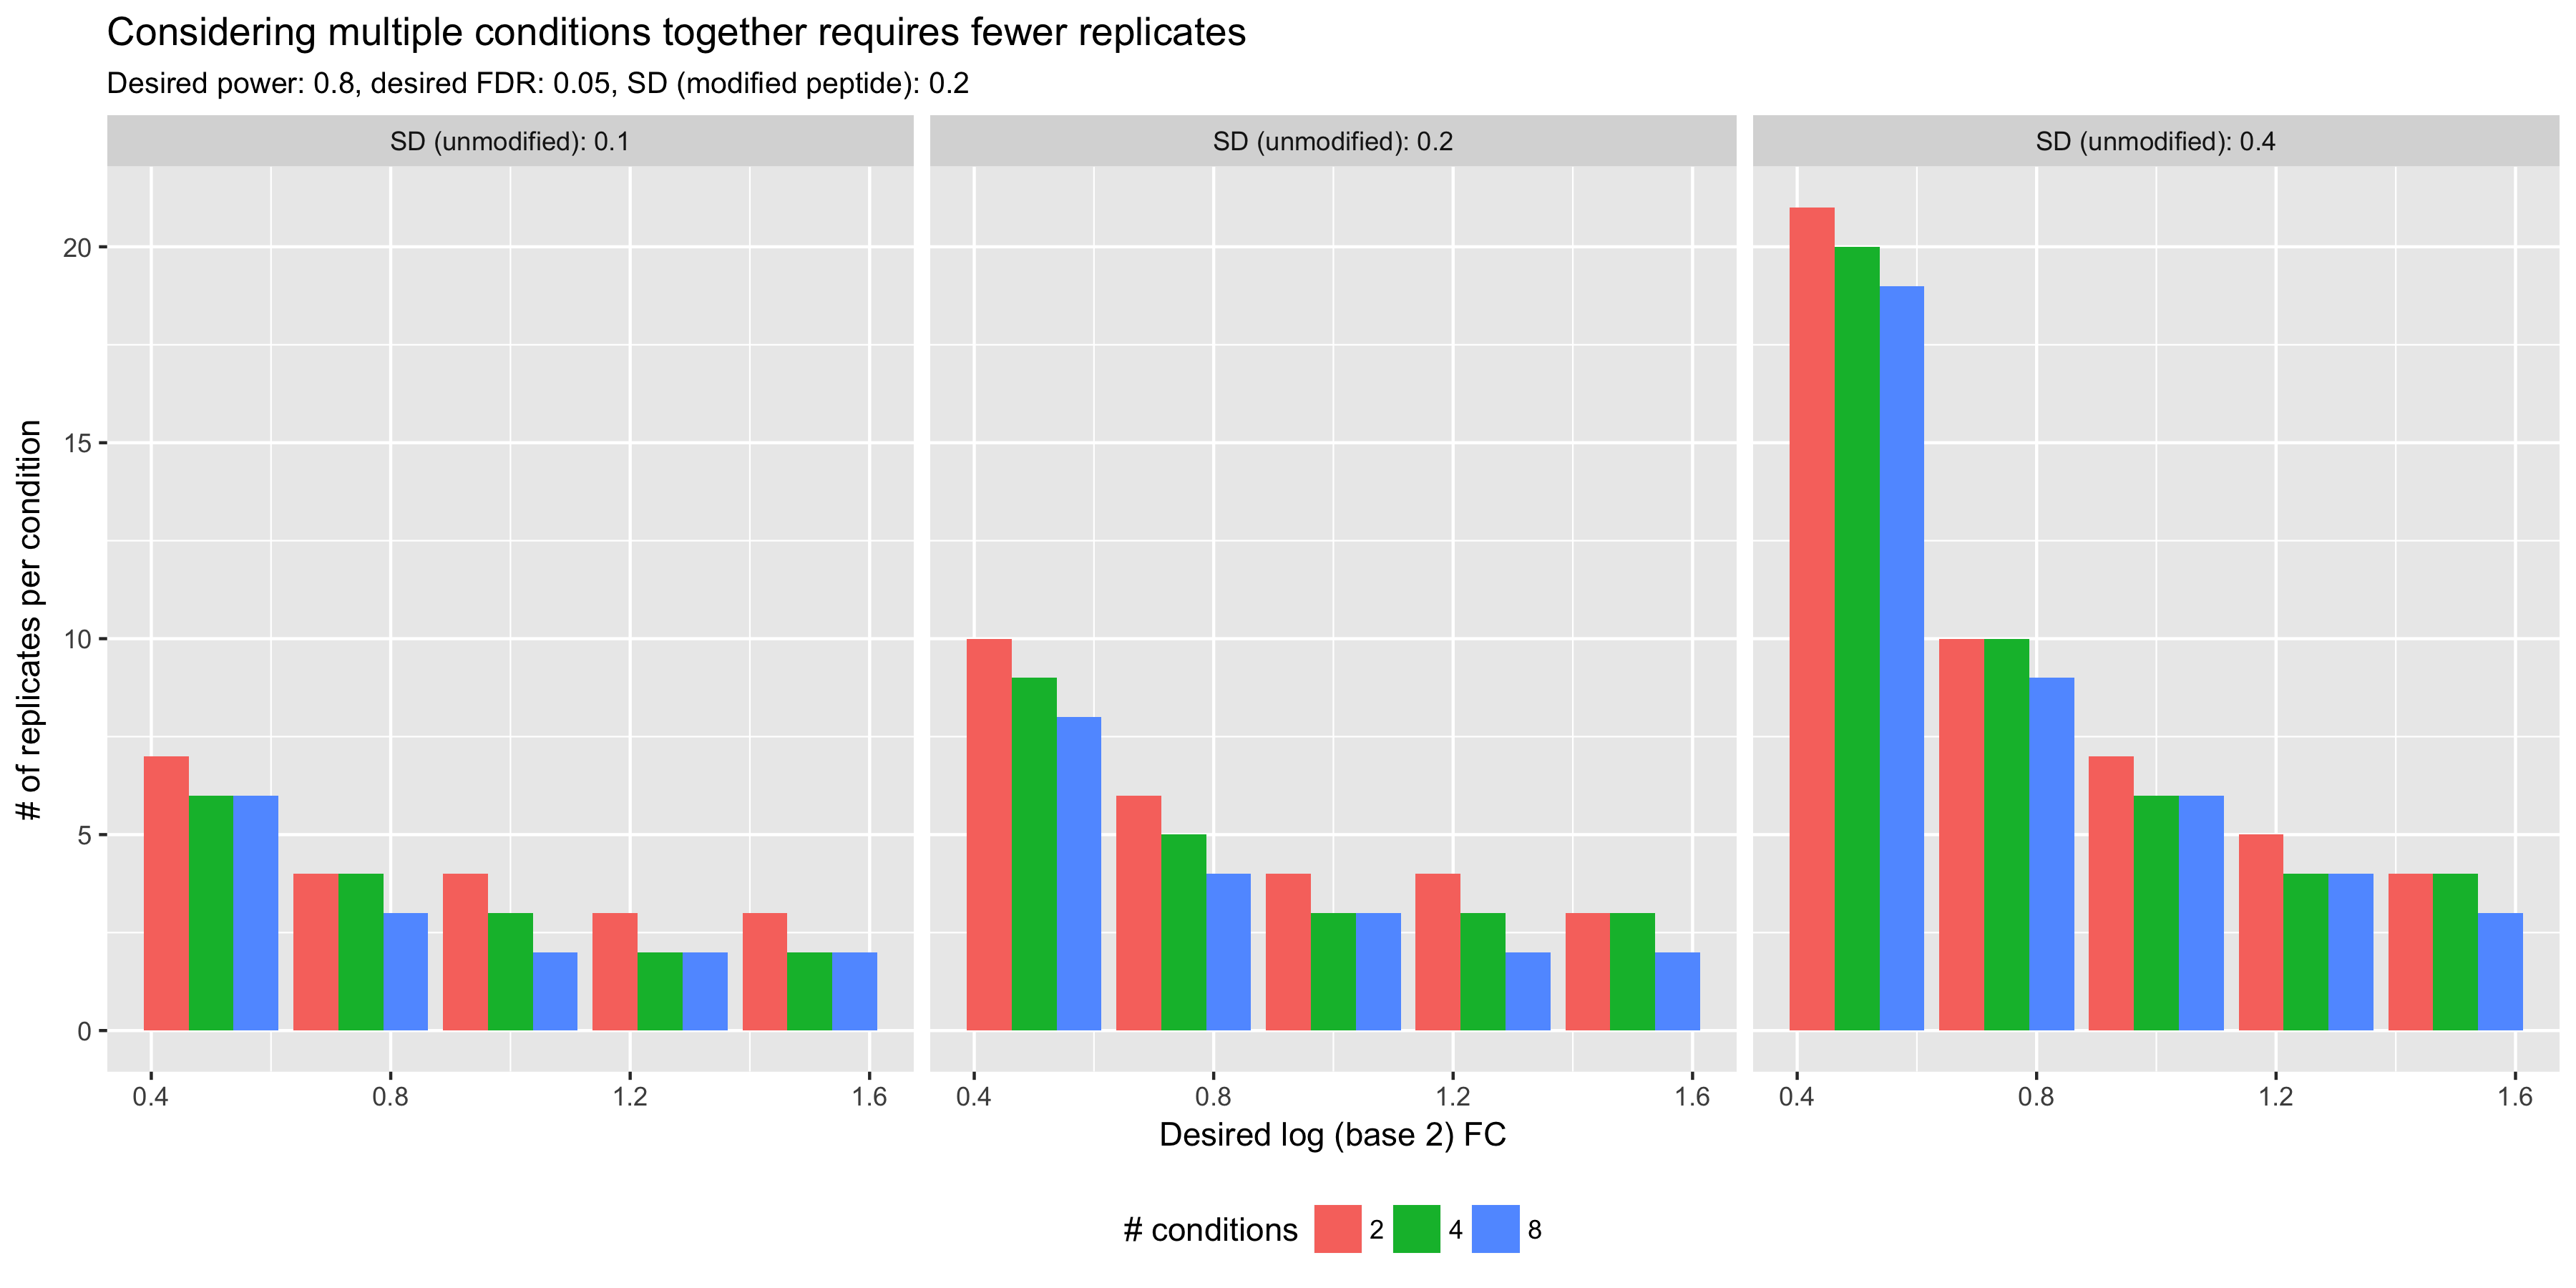
\includegraphics[width=.725\textwidth]{sim/size_grp}
%\caption{In complex designs, simultaneously analyzing all the conditions% effectively increases the degrees of freedom and requires fewer replicates. %\label{fig:size_grp}}
%\end{figure}

%\begin{figure}[h!]
%\centering
%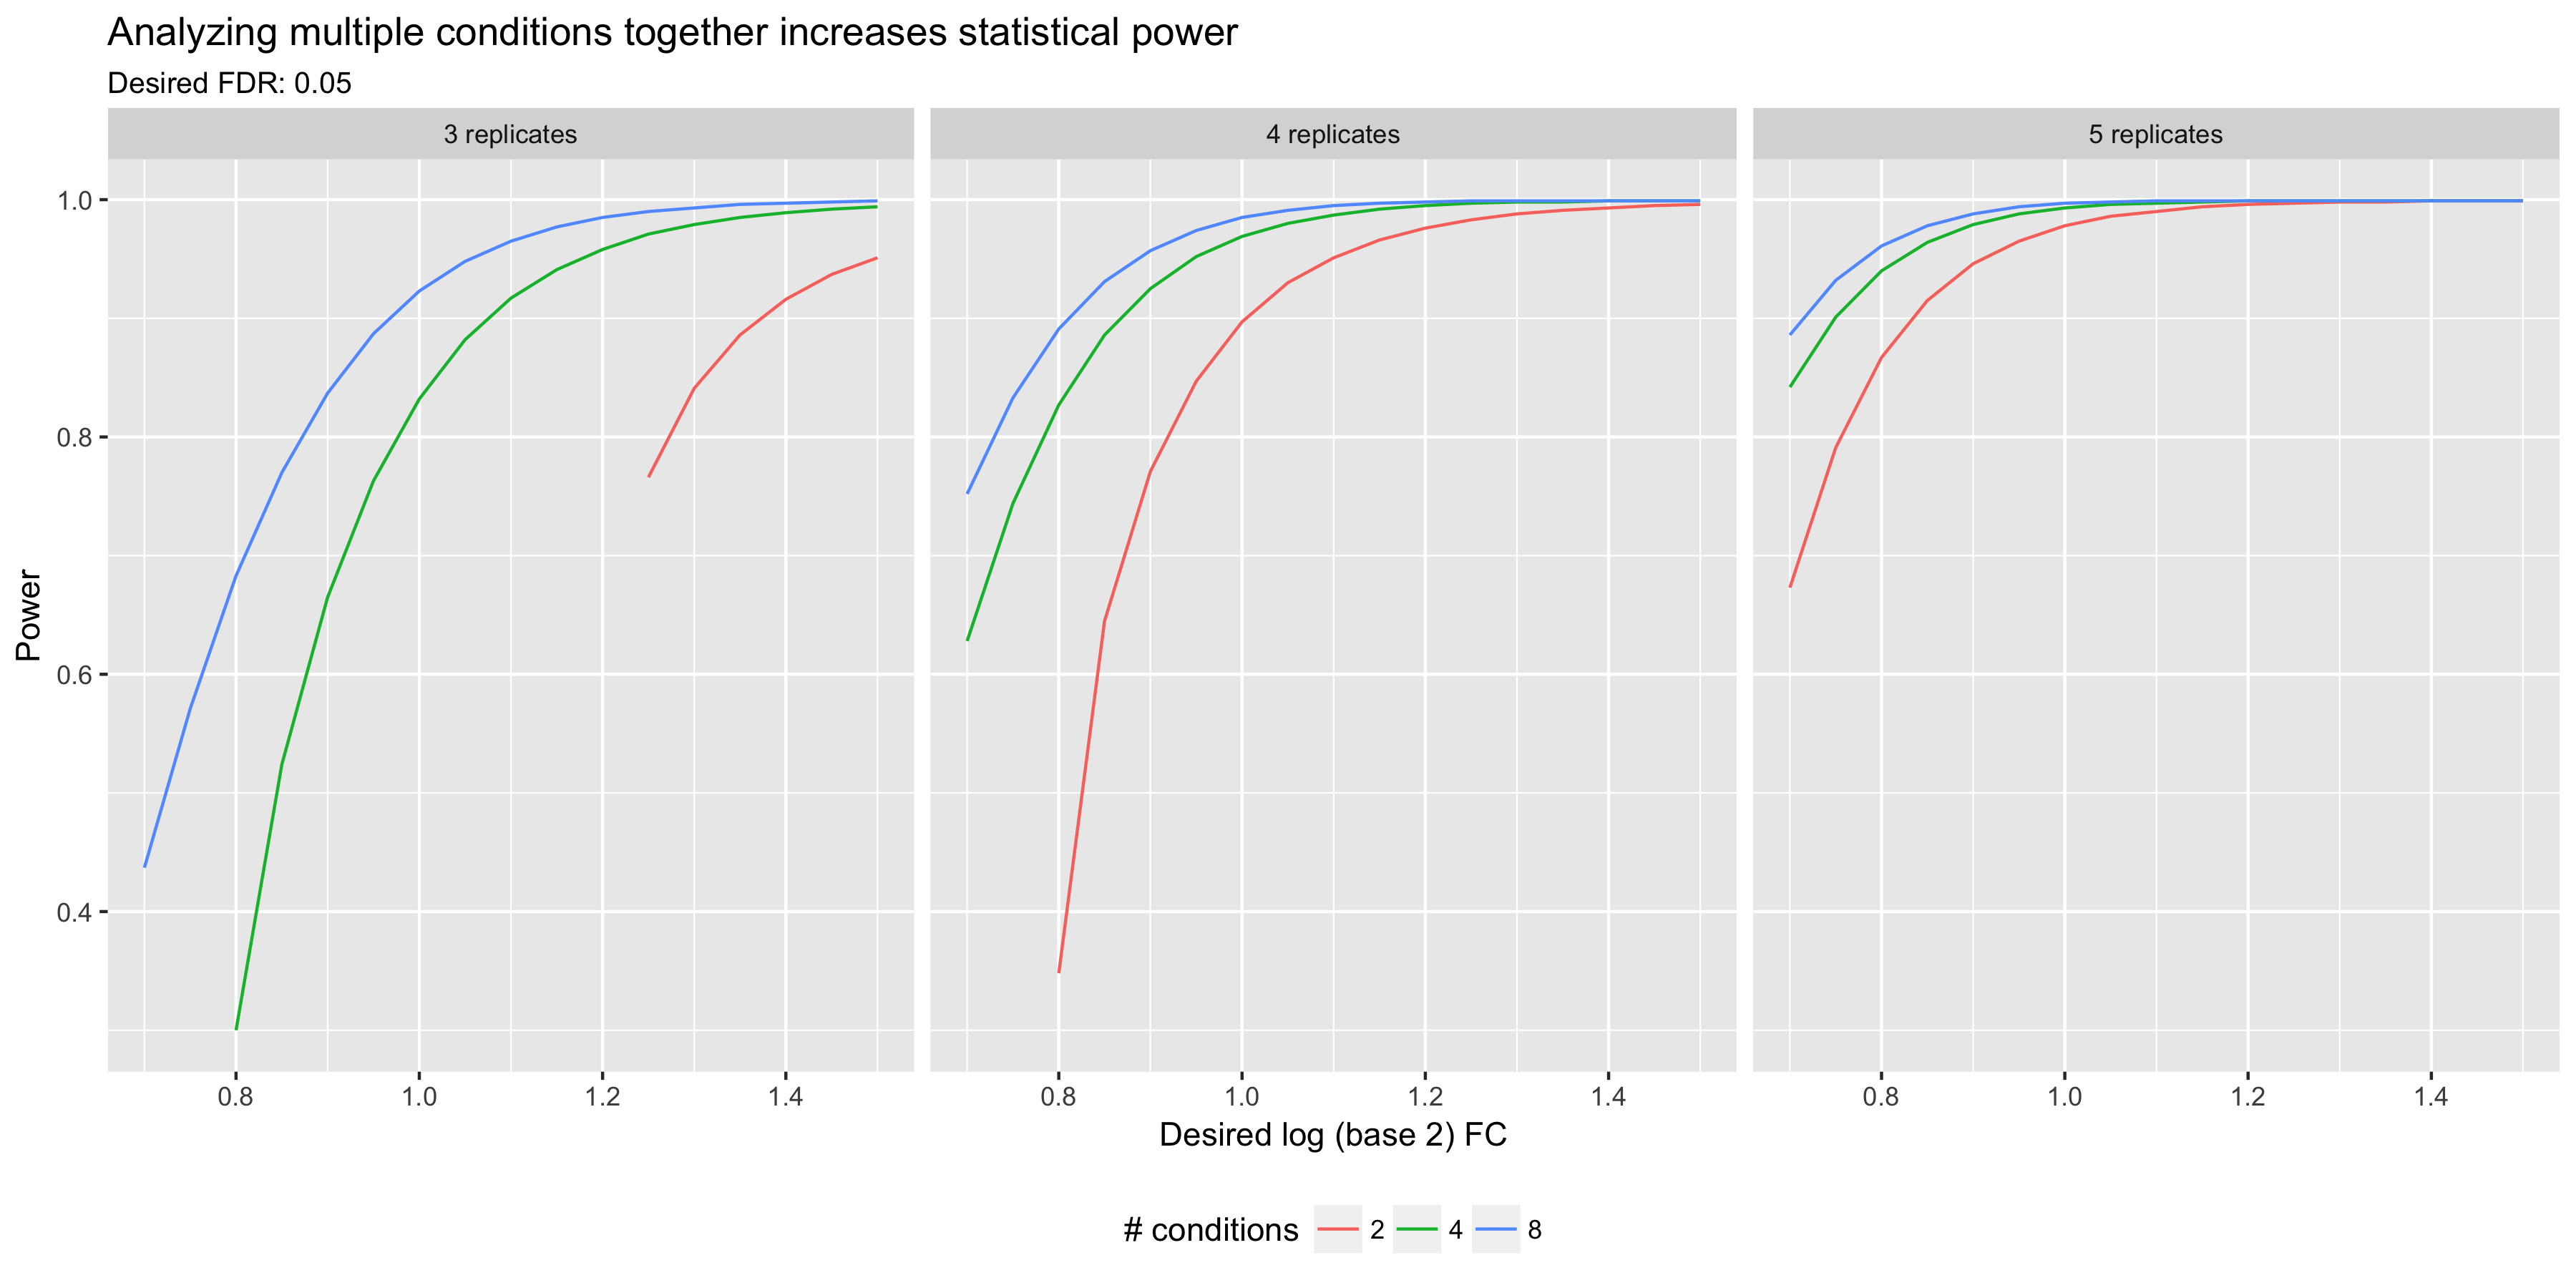
\includegraphics[width=\textwidth]{sim/pwr_grp}
%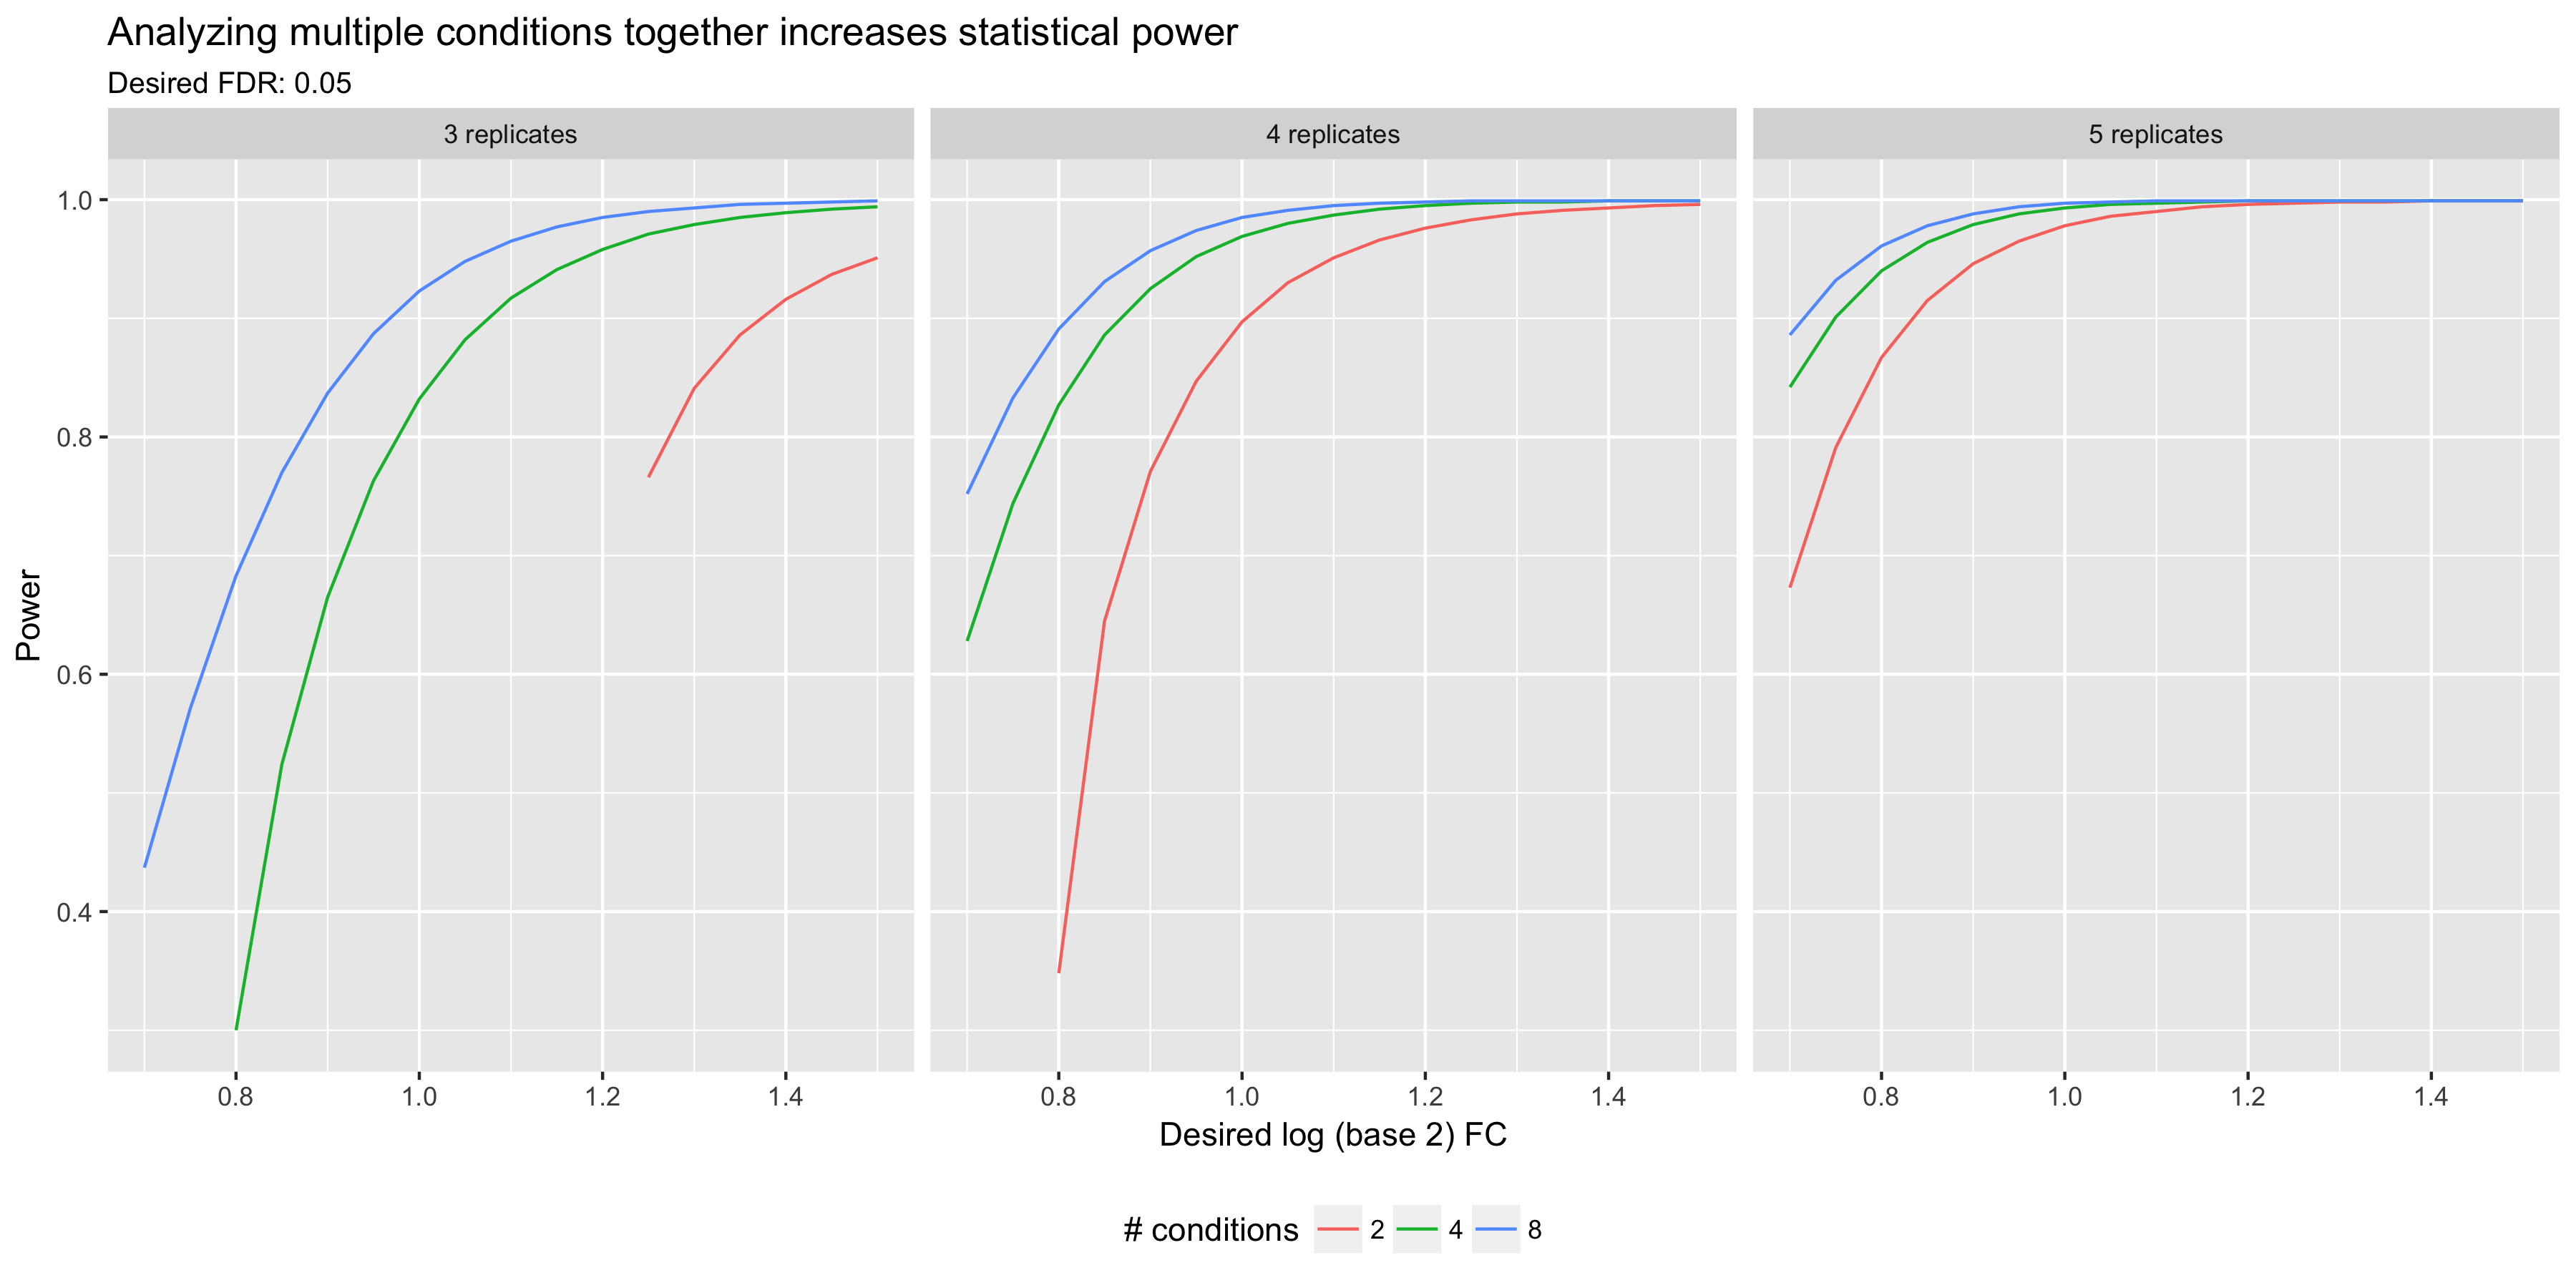
\includegraphics[width=.725\textwidth]{sim/pwr_grp}
%\caption{Statistical power can be improved by increasing the sample size and %analyzing multiple conditions together. \label{fig:pwr_grp}}
%\end{figure}



%%%%%%%%%%%%%%%%%%%%%%%%%%%%%%%%%%%%%%%%%%%%%%%%%%%%%%%%%%%%%%%%
\clearpage

\todo{move to main manuscript}

\section{Further Considerations}

\subsubsection{Multiple sites per protein}

Expression levels of PTM sites are adjusted based on the abundance of their originating protein. Since the same reference is used for all sites, it introduces correlation among estimates and test statistics for those sites. This may cause issues in controlling false discovery rate (FDR).
We investigated the property by simulating data of two conditions and 1000 proteins with different numbers of PTM sites and comparing the results of the proposed approach and the linear model with no adjustment. 
%We investigated the property by simulating data of two conditions and 1000 proteins with different numbers of PTM sites. 
A fraction (50\%) of the 1000 proteins had no changes between conditions while systematic changes were simulated for the rest of the proteins. Multiple testing correction was performed using the Benjamini and Hochberg's method. 
Performances of the considered approaches were assessed by their actual FDR, calculated as the fraction of proteins with adjusted $p$-values $<0.05$ among the proteins with true differences. The results are summarized in \sfigref{fig:prot_fdr}.
%Performances of the considered approaches were assessed by their power and FDR. The power was calculated as the fraction of proteins with adjusted $p$-values $<0.05$ among those proteins with true differences between conditions, while the FDR was calculated as the fraction of proteins with adjusted $p$-values $<0.05$ among the proteins with true differences. The results are summarized in \sfigref{fig:prot_fdr}.

%%%%%%%%%%%%%%%%%%%%%%%%%%%%%%%%%%%%%%%%%%%%%%%%%%%%%%%%%%%%%%%%%
\clearpage
\section*{References}

\bibliographystyle{plain}
\bibliography{ptm_ref}

\end{document} 

